\documentclass[12pt, a4paper]{report}

\usepackage{authblk}
\usepackage{graphicx}
\usepackage{hyperref}
\usepackage{blindtext}
\usepackage{placeins}
\usepackage{array}

\hypersetup{
    colorlinks=true,
    linkcolor=blue,
    filecolor=magenta,      
    urlcolor=cyan,
    pdftitle={User Manual },
    pdfpagemode=FullScreen,
    }

\graphicspath{ {./images/} }

\begin{document}

\title{Reverse Computational Research Hub Group 19}
\author[1]{Klaudiusz D. Halek}
\author[1]{Mason Hariness}
\author[1]{Hugo Hull}
\author[1]{Josh J. Hull}
\author[1]{Alex A. Martin}
\author[1]{Lee Milligan}
\author[1]{Artemis J. Roberts}
\author[1]{Teodor Sula}
\affil[1]{University of Leicester}
\date { }
\maketitle

\tableofcontents
\clearpage

\chapter{What is the Purpose of this Application?}
The reverse computation research hub serves as a website for researchers and laypeople to come together and learn, read, and discuss topics of reverse computation. Users can share and view publications of pdf format, create posts for events, and share general updates. along with functionality for automatic keyword searching for publications and events. The user can view and sample pseudocode in forward and reverse direction.
Previously, alot of this collaboration would be done using primitive methods that limited people in the fields ability to communicate. The goal of this website is to fix that problem.

\chapter{How to Get Started}
The user starts on the homepage, signed out. In this signed-out state, the user can view the homepage, providing a brief introduction to the website and the field of reverse computation.
The user can also view publications and events by navigating to their relevant page via the nav bar at the top of the page.
A simulator is also available to all users that can run code snippets in an online environment.

\begin{figure}[h]
	\centering
	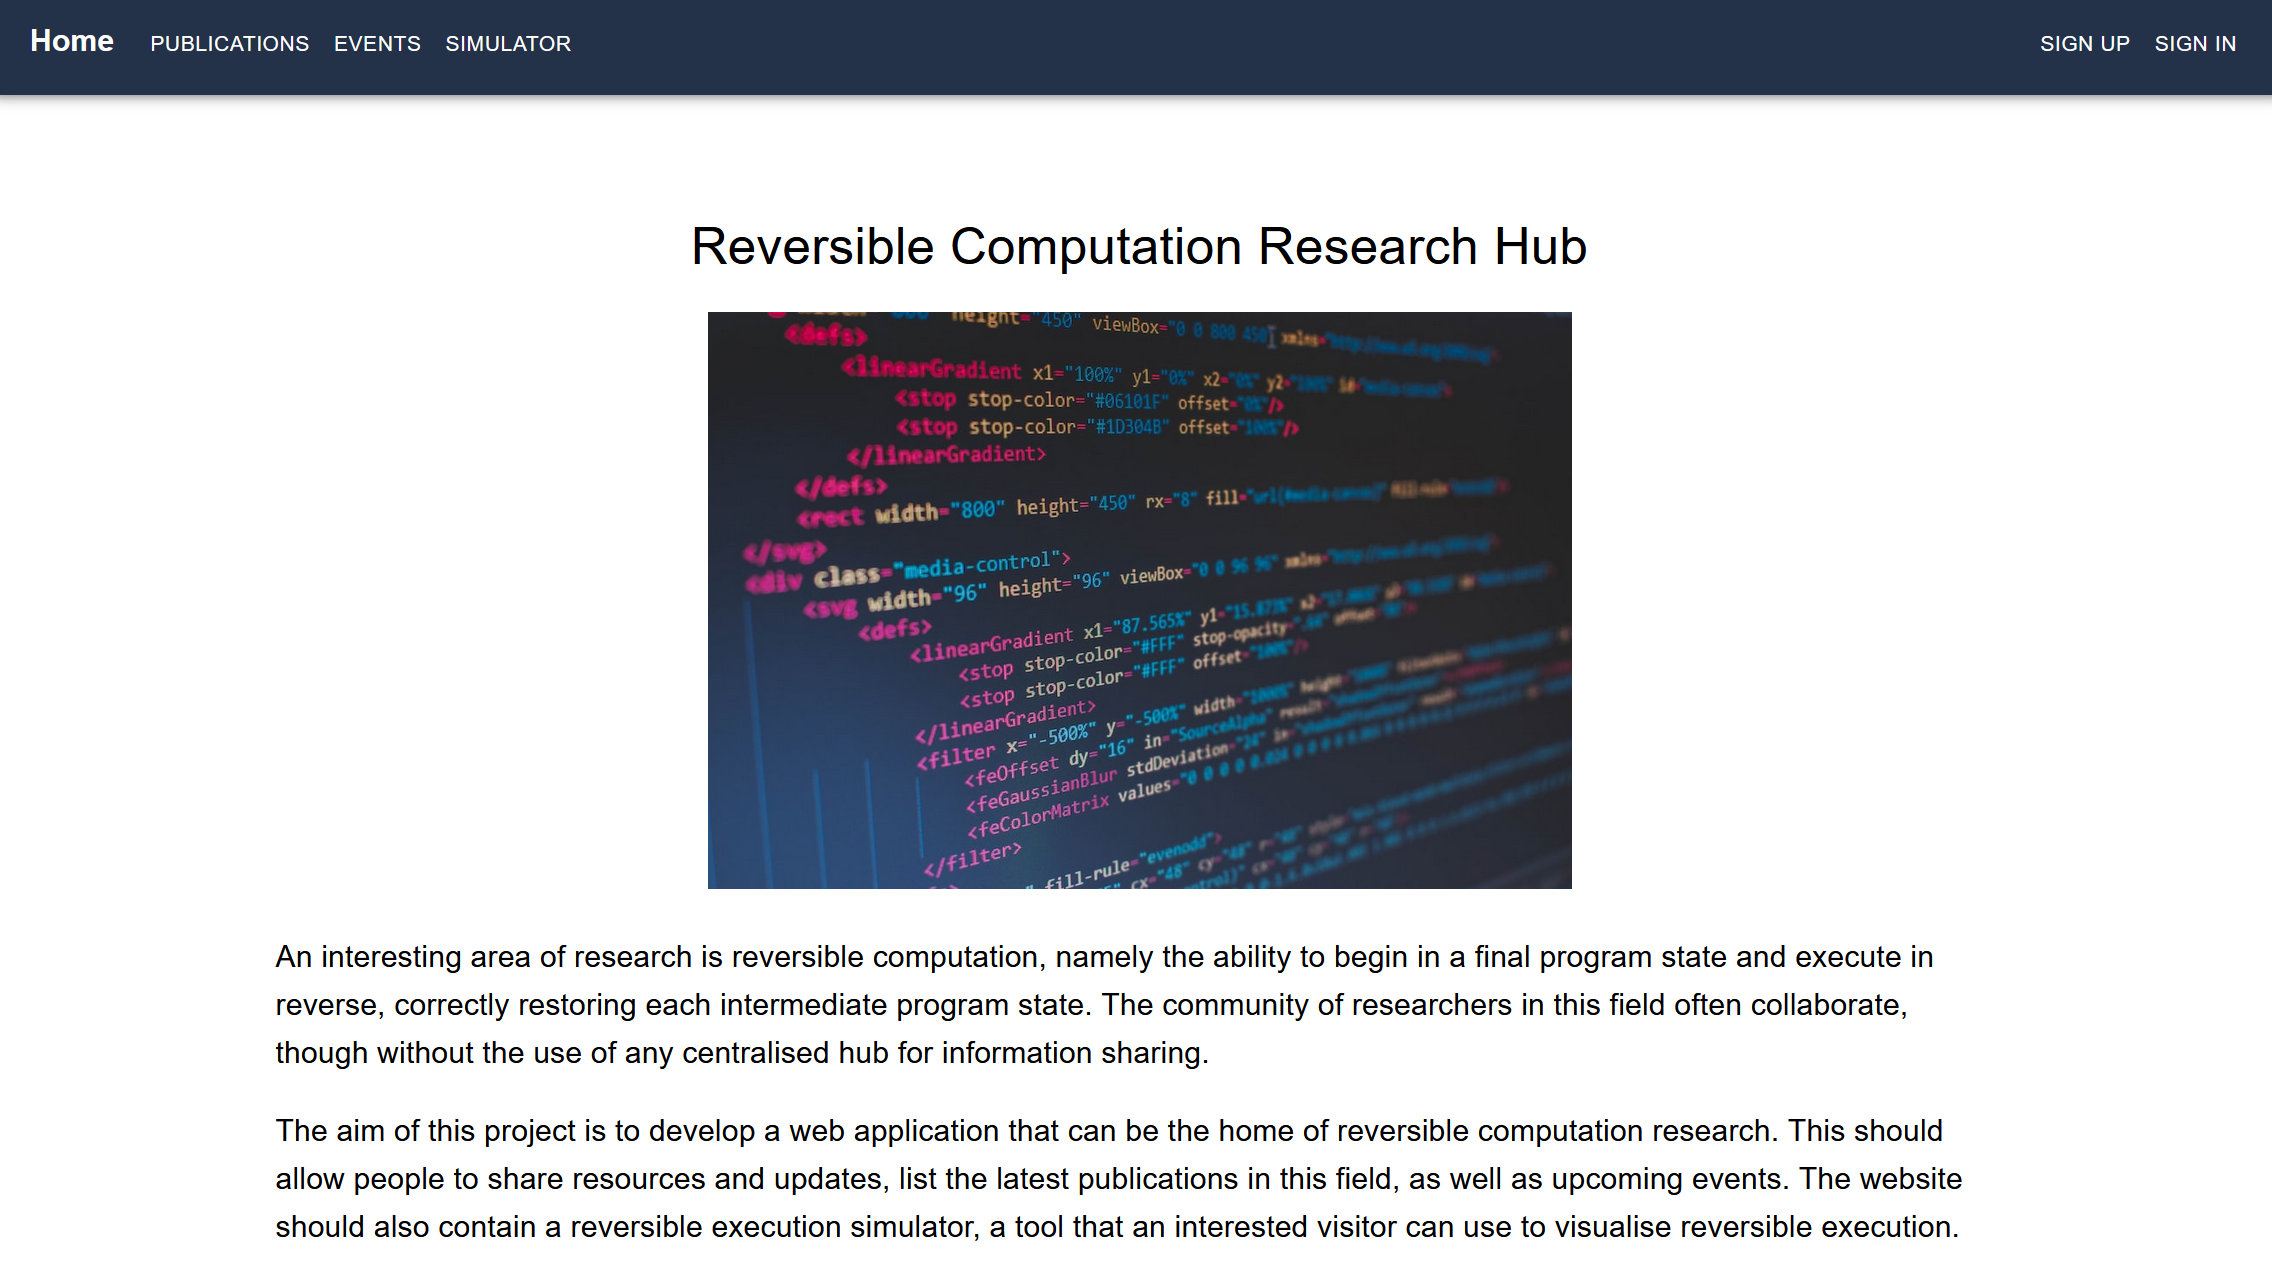
\includegraphics[width=\textwidth]{MainPage}
	\caption{Homepage for Signed-out Users}
\end{figure}

\newpage
\section{Sign-up}

To access full functionality, the user must be signed into an account. If they do not have an exisitng account they can create one by clicking on the sign-up button on the navigation bar.

\begin{figure}[h]
	\centering
	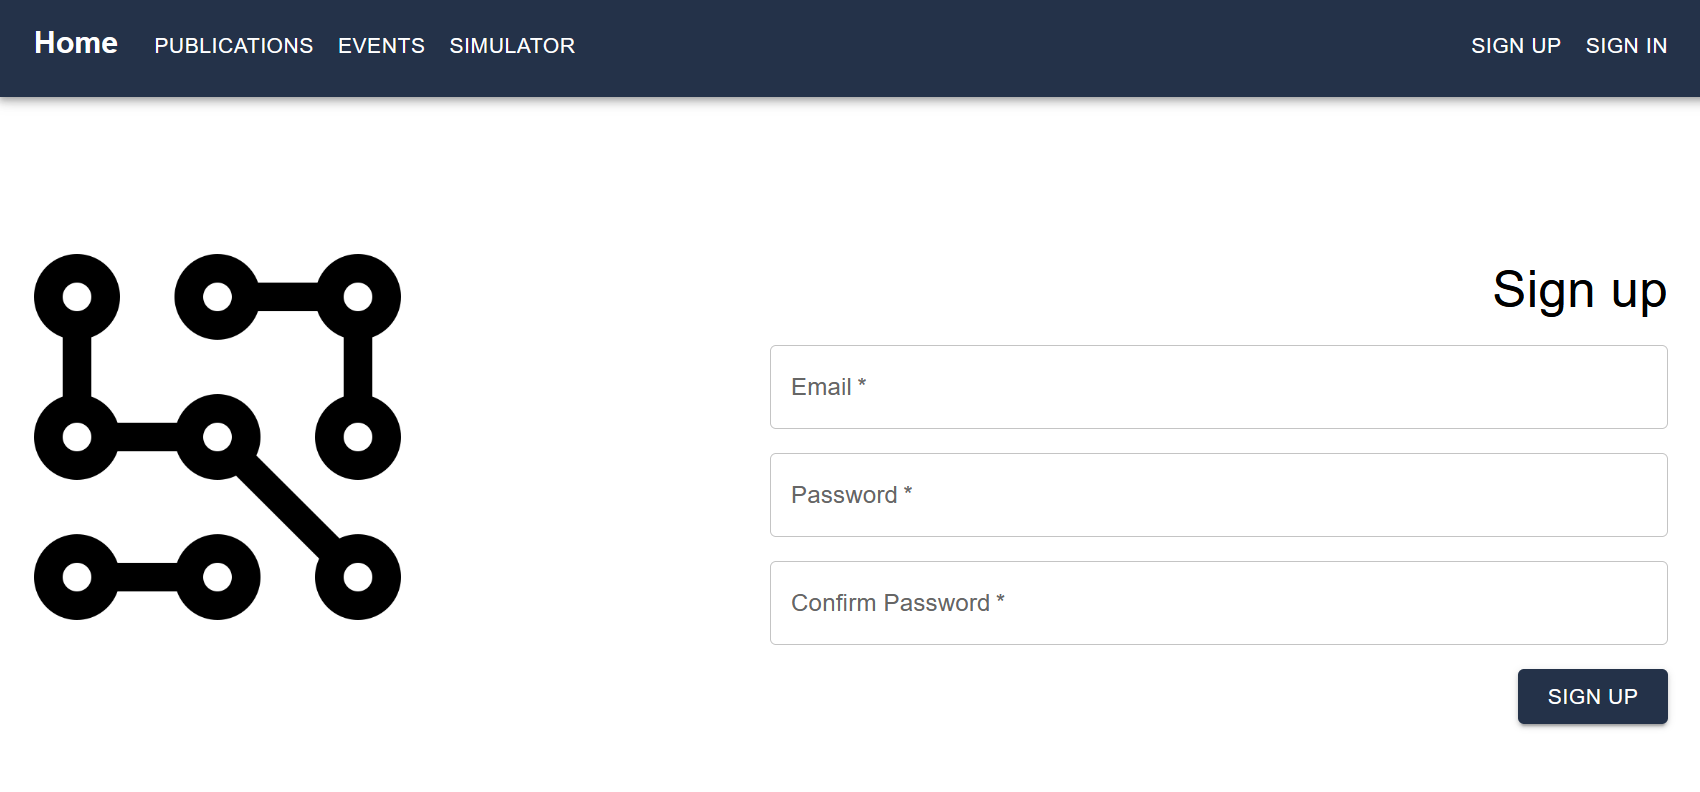
\includegraphics[width=\textwidth]{SignUpPage}
	\caption{Sign-up page}
\end{figure}

\newpage
\section{Errors in Sign-up}

If an error occurs with the information inputted, it will be displayed on the webpage. This can then be used by the user to fix the error.

\subsection{Missing Value}
This indicates that there is a value missing in one of the input fields. The fields described will be flagged and can be fixed by adding valid information.

\begin{figure}[h]
	\centering
	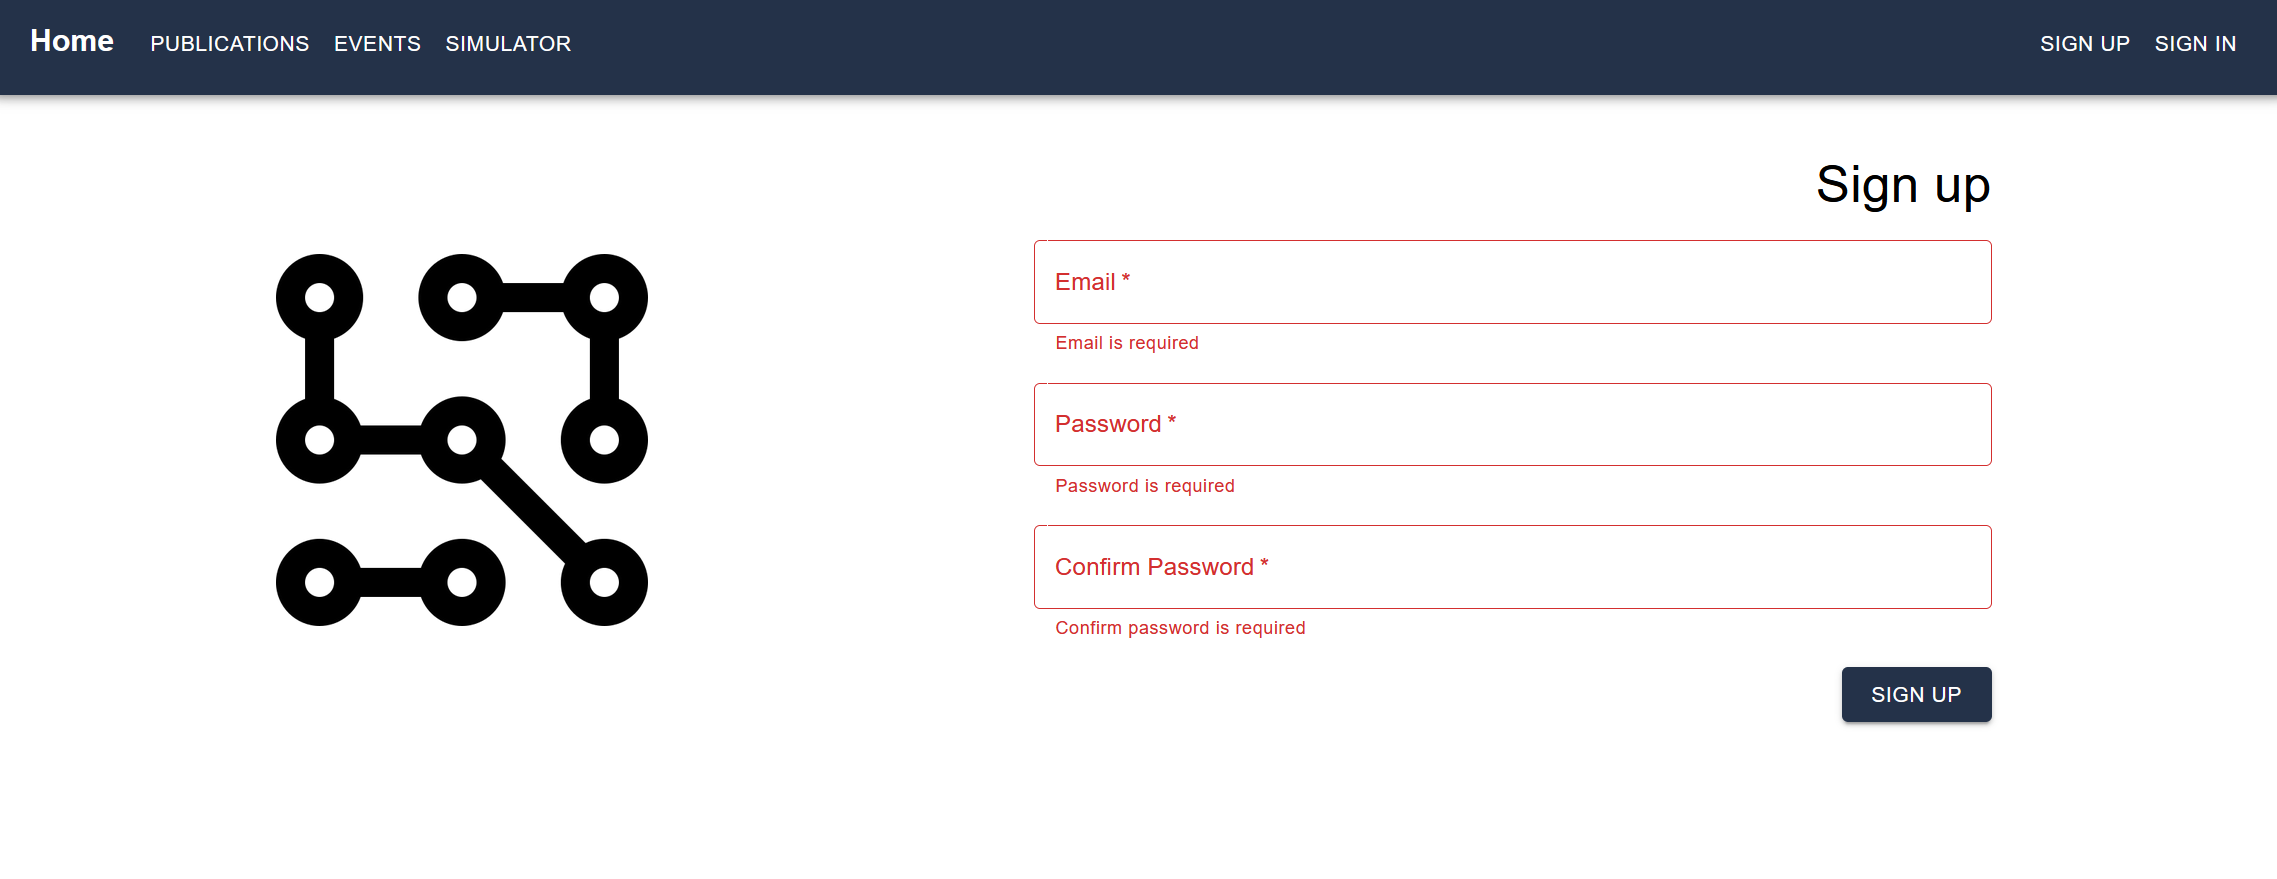
\includegraphics[width=\textwidth]{SignUpPageMissingValue}
	\caption{Values are missing and need to be entered}
\end{figure}

\newpage
\subsection{Invalid Email}
This occurs when the email entered is not a valid email. This can be fixed by ensuring the information inputted is correct.

\begin{figure}[h]
	\centering
	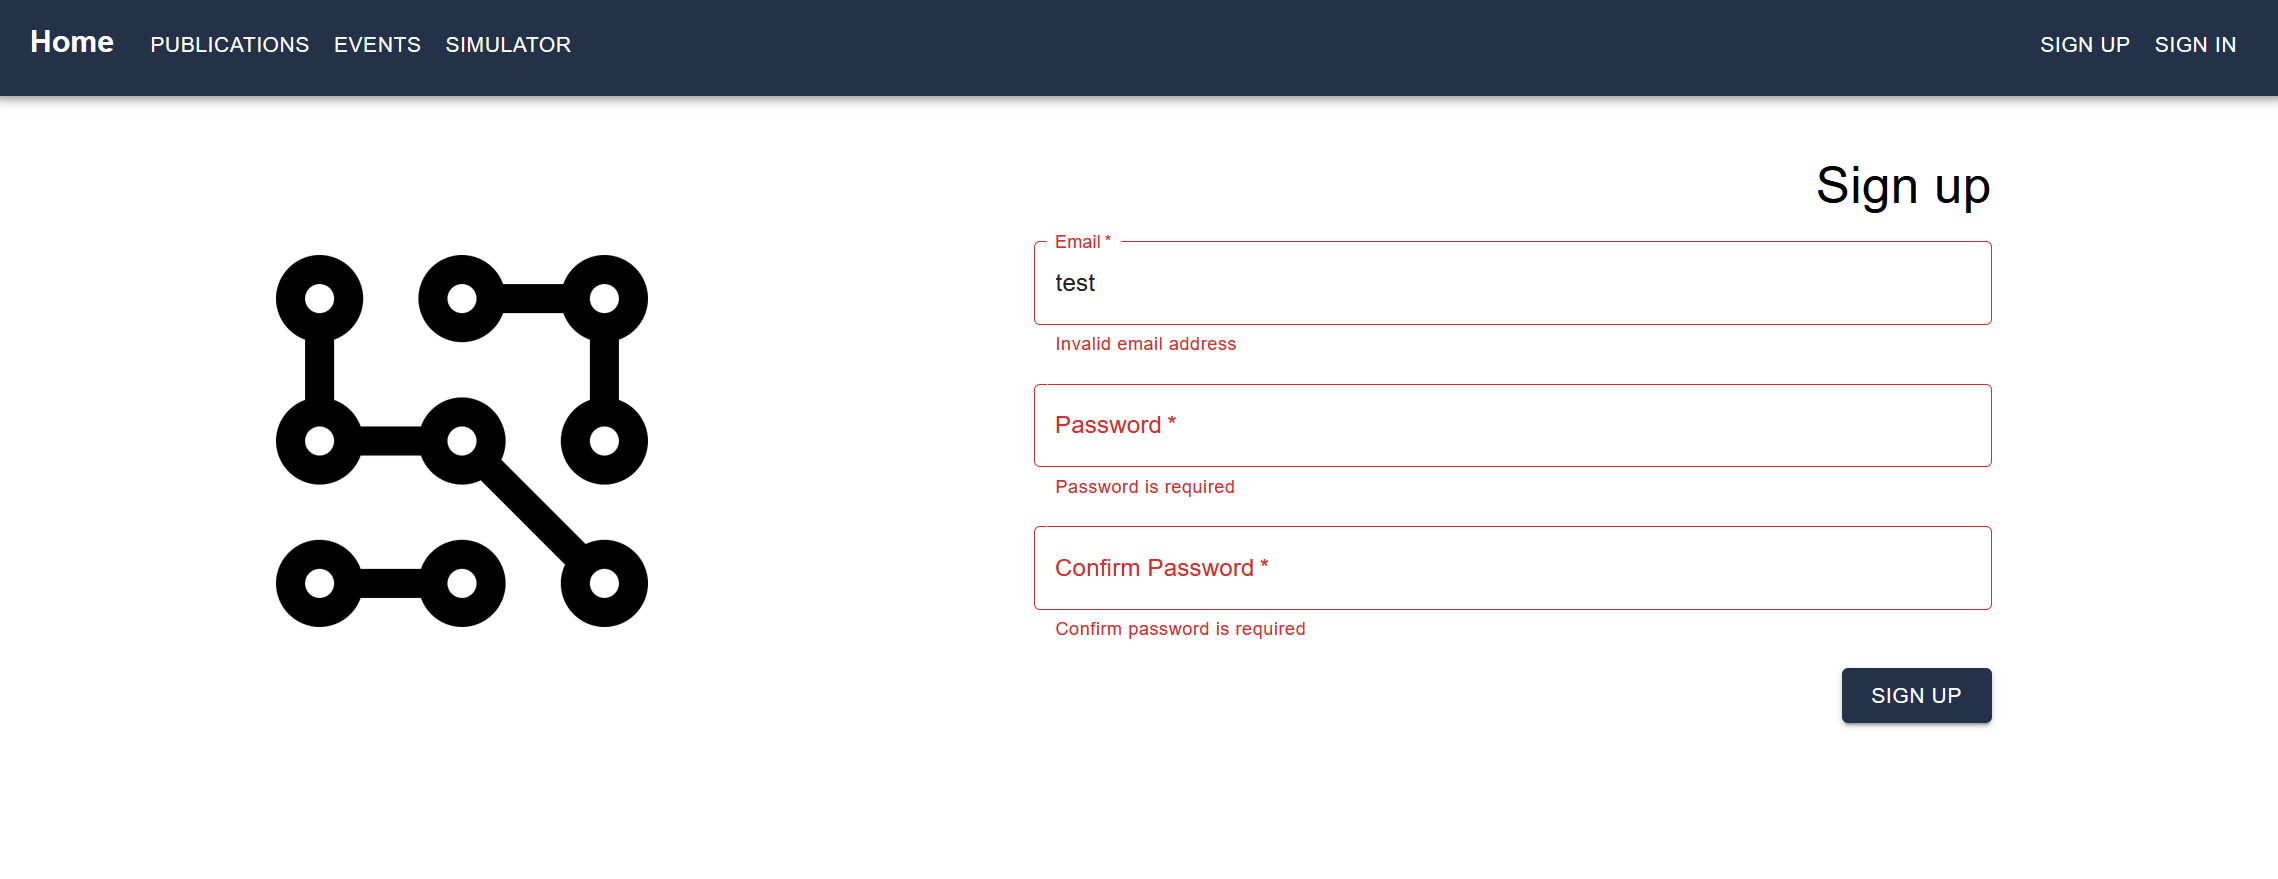
\includegraphics[width=\textwidth]{SignUpPageInvalidEmail}
	\caption{The email entered is not a valid email and needs changing}
\end{figure}

\newpage
\subsection{Invalid Password}
This occurs when the password inputted does not conform to the required character security rules.

\begin{figure}[h]
	\centering
	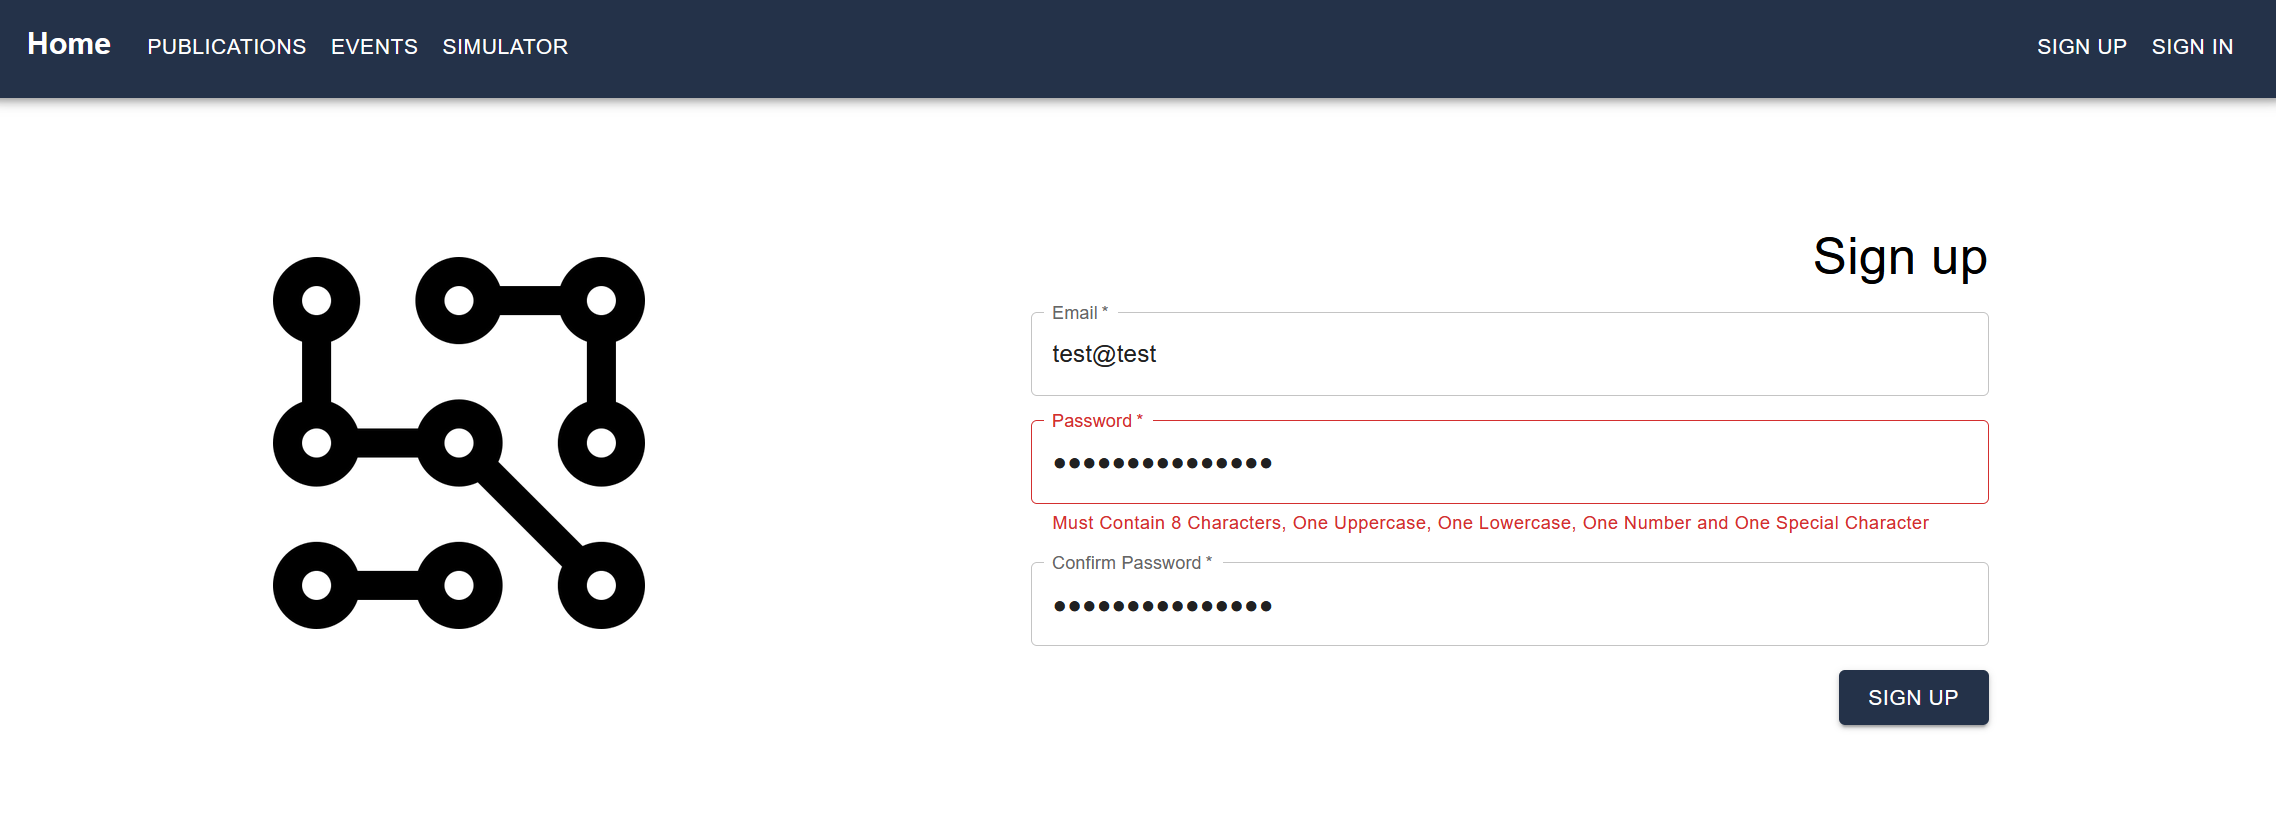
\includegraphics[width=\textwidth]{SignUpPagePasswordError}
	\caption{Password needs additional characters}
\end{figure}

\newpage
\subsection{Miss-matched Password}
This occurs when the passwords entered into the sign-up page do not match. The user should check to ensure both entries of the password match to fix this error.

\begin{figure}[h]
	\centering
	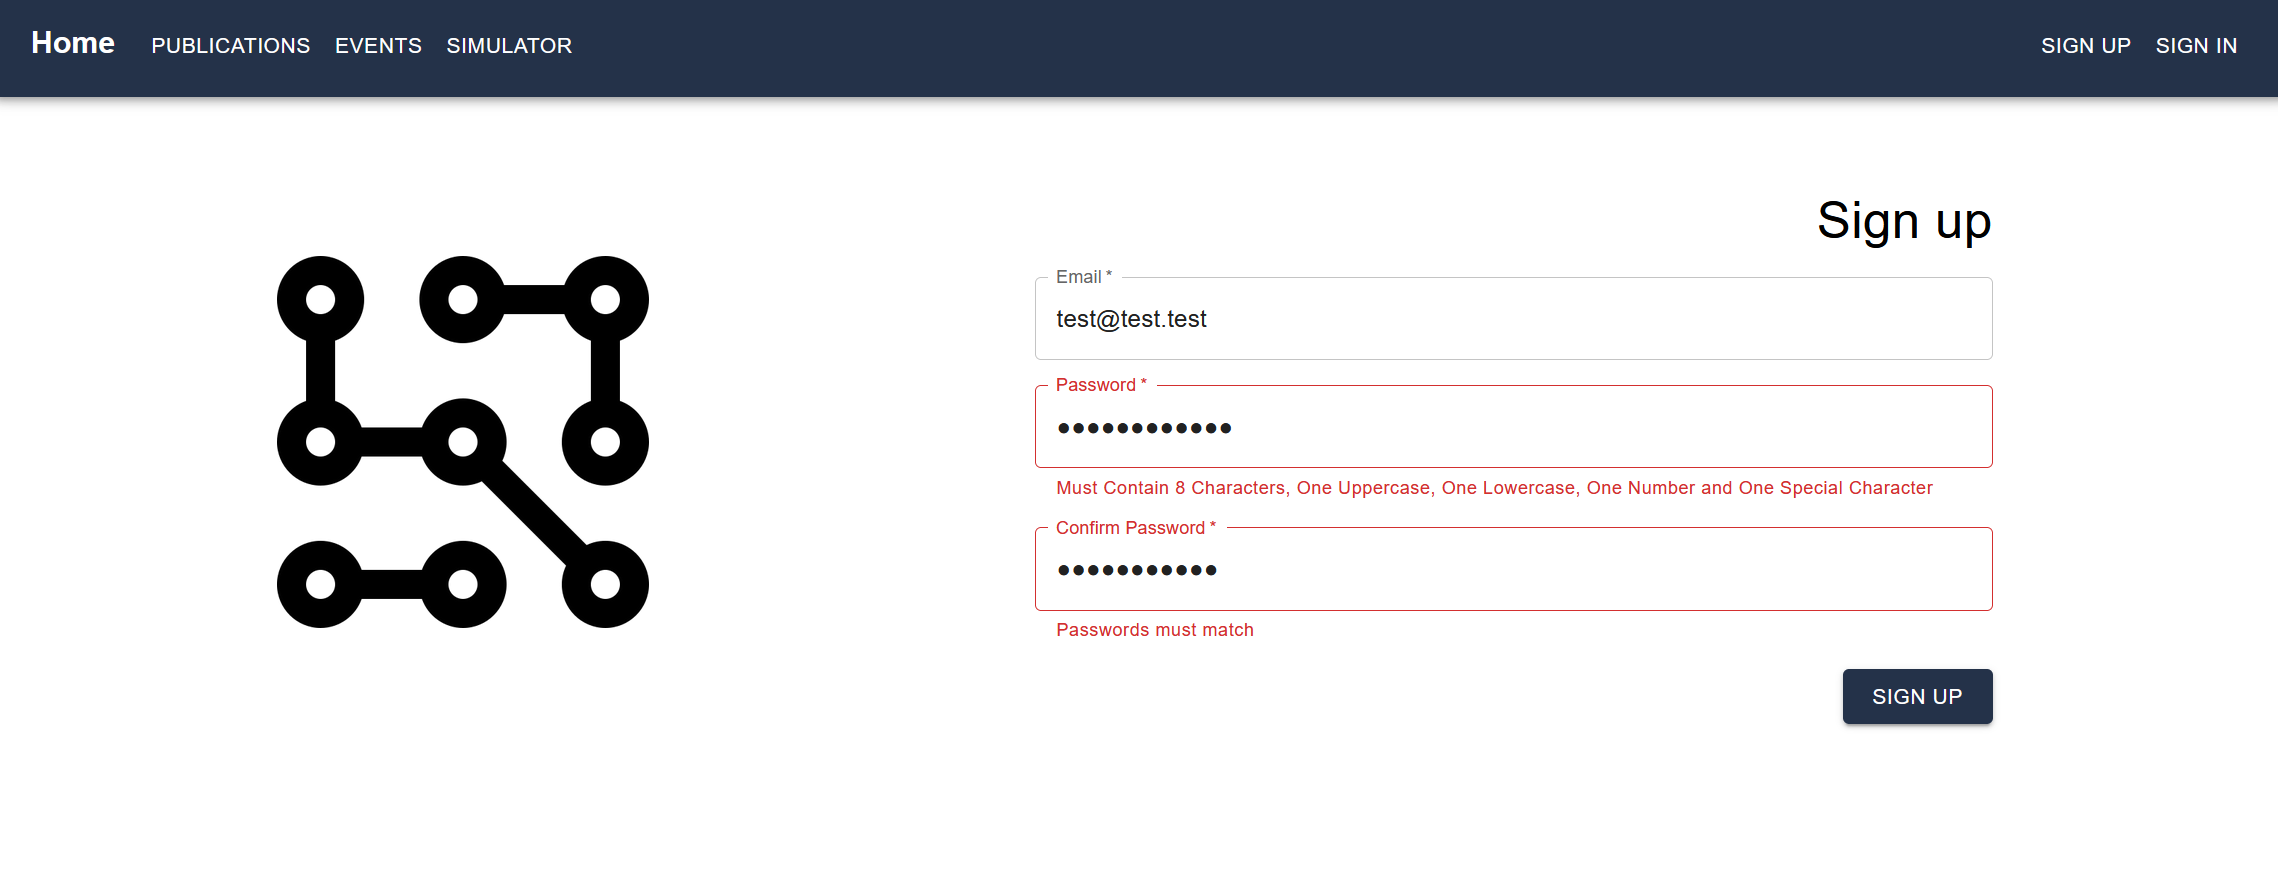
\includegraphics[width=\textwidth]{SignUpPagePasswordMatching}
	\caption{Passwords do not match}
\end{figure}

\newpage
\section{After Account Creation}

The user can enter an email \& password to use for their account, and they can then click the ‘sign up’ button to finish. After this, the user can navigate to the homepage and have access to full functionality. The user can logout to revert to the sign-in page.

\begin{figure}[h]
	\centering
	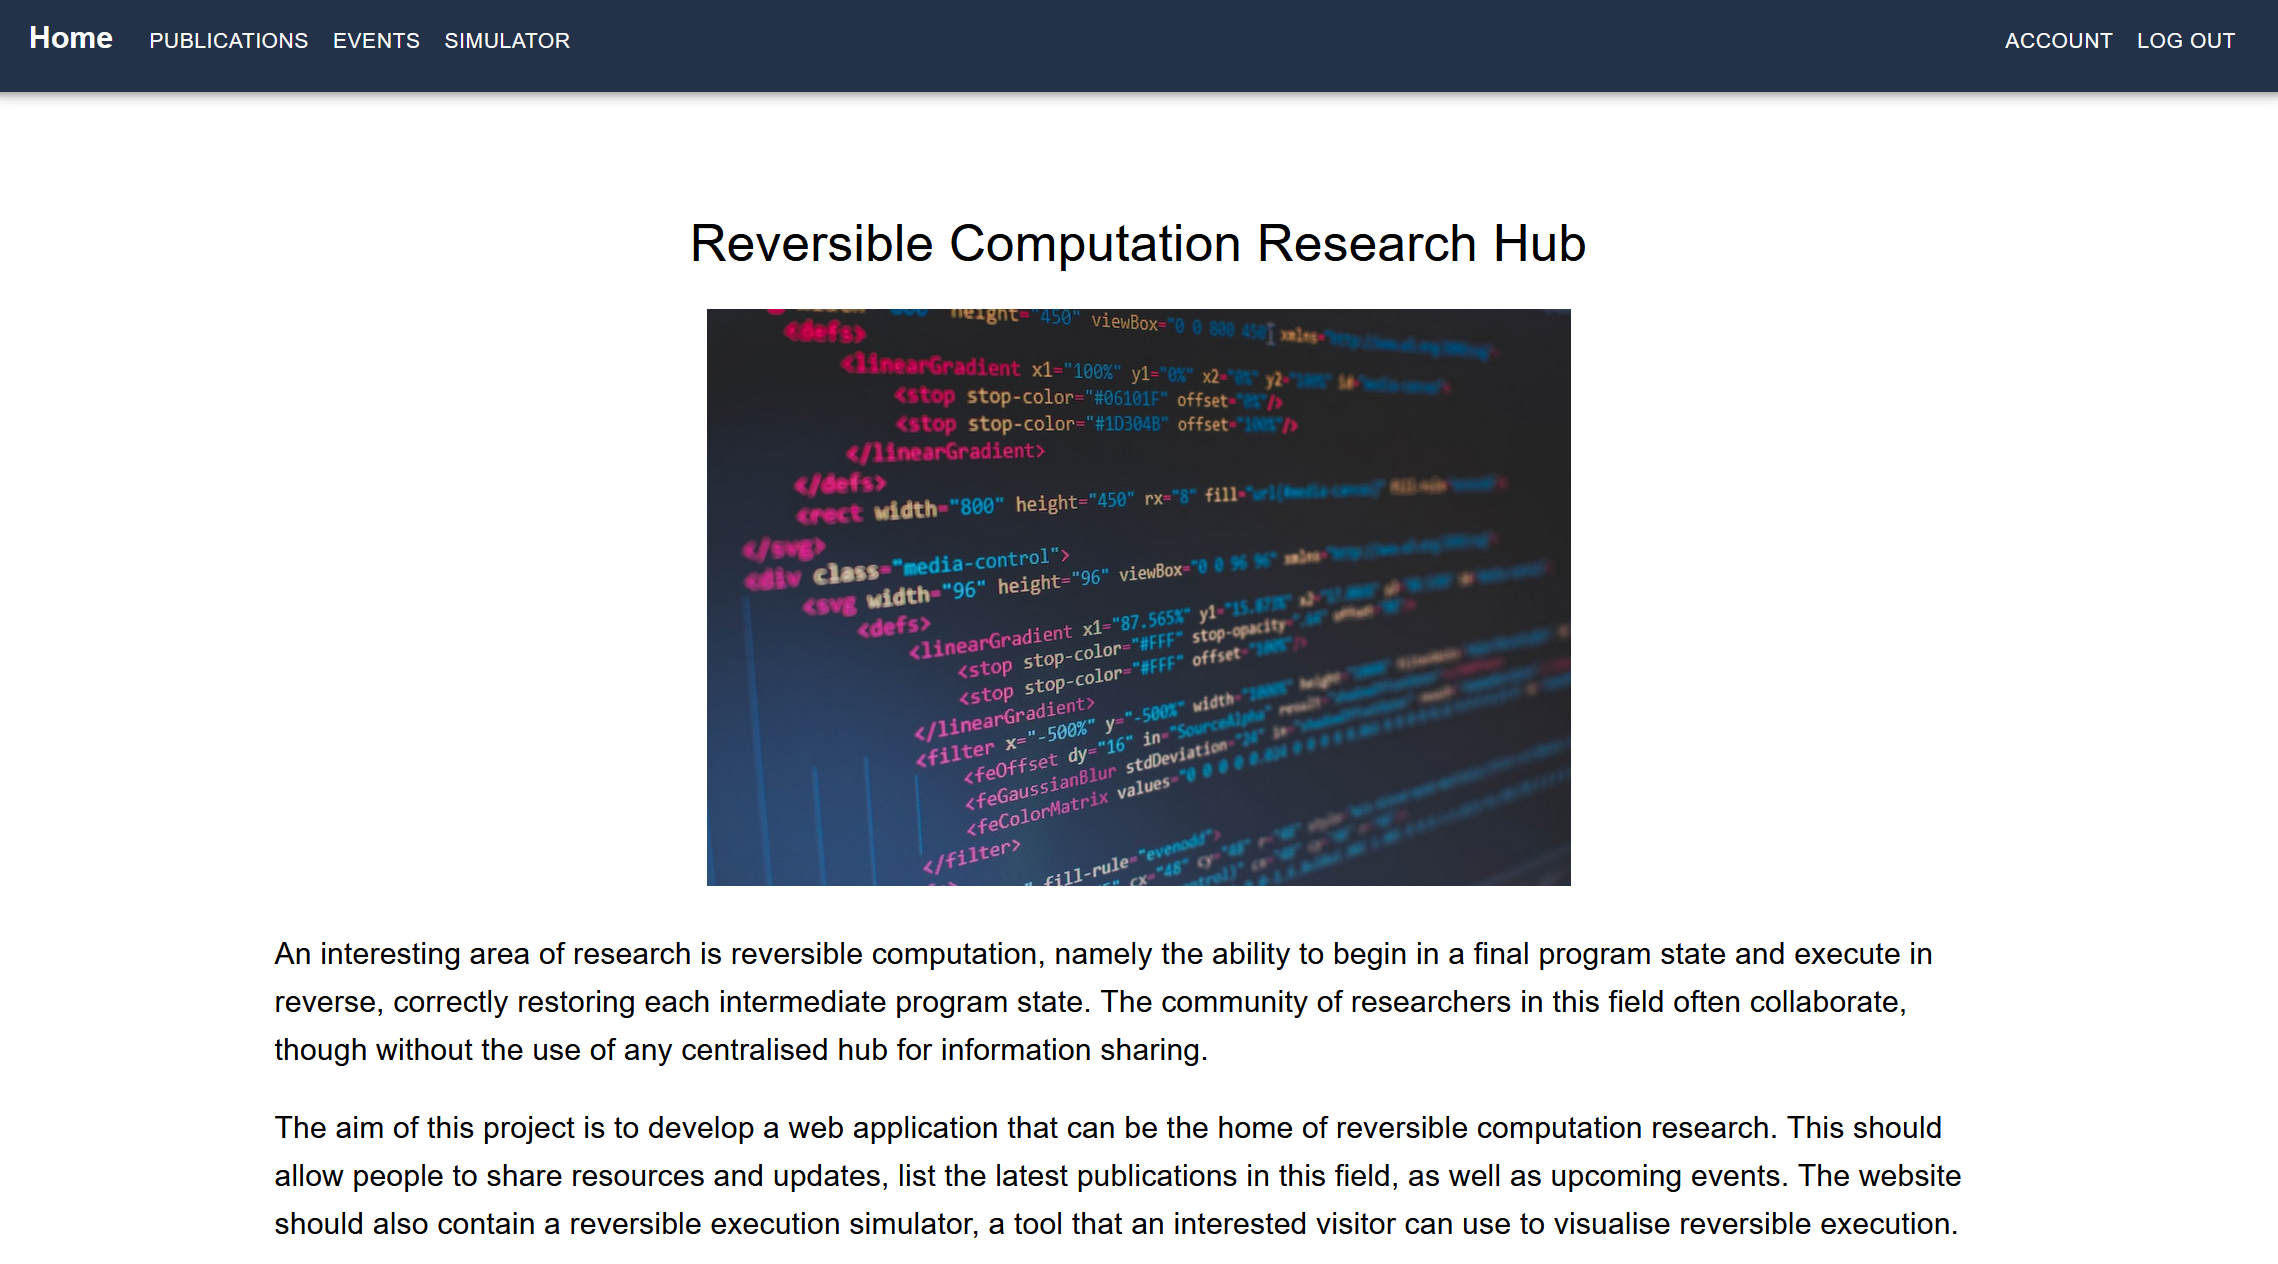
\includegraphics[width=\textwidth]{MainPageLoggedIn}
	\caption{Homepage for logged-in users}
\end{figure}

\newpage
\section{Sign-in}

If the user wishes to sign-in using their details, they can now use the sign-in button at the top.

\begin{figure}[h]
	\centering
	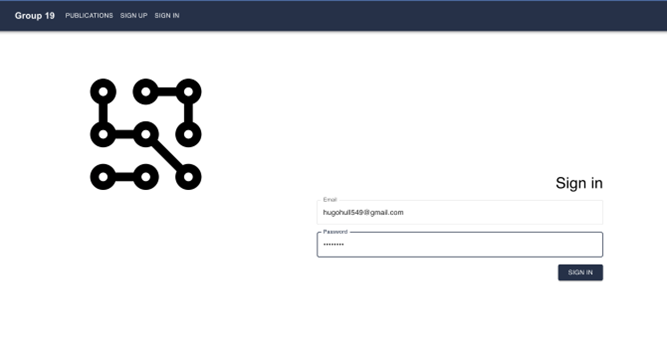
\includegraphics[width=\textwidth]{Picture4}
	\caption{Sign-in page}
\end{figure}


\newpage
\section{Errors in Sign-in}

If an error occurs with the information inputted, it will be displayed on the webpage. This can then be used by the user to fix the error.

\subsection{Value is Required}
This indiates that there is a value missing in one of the input fields. The fields described will be flagged and can be fixed by adding valid information.

\begin{figure}[h]
	\centering
	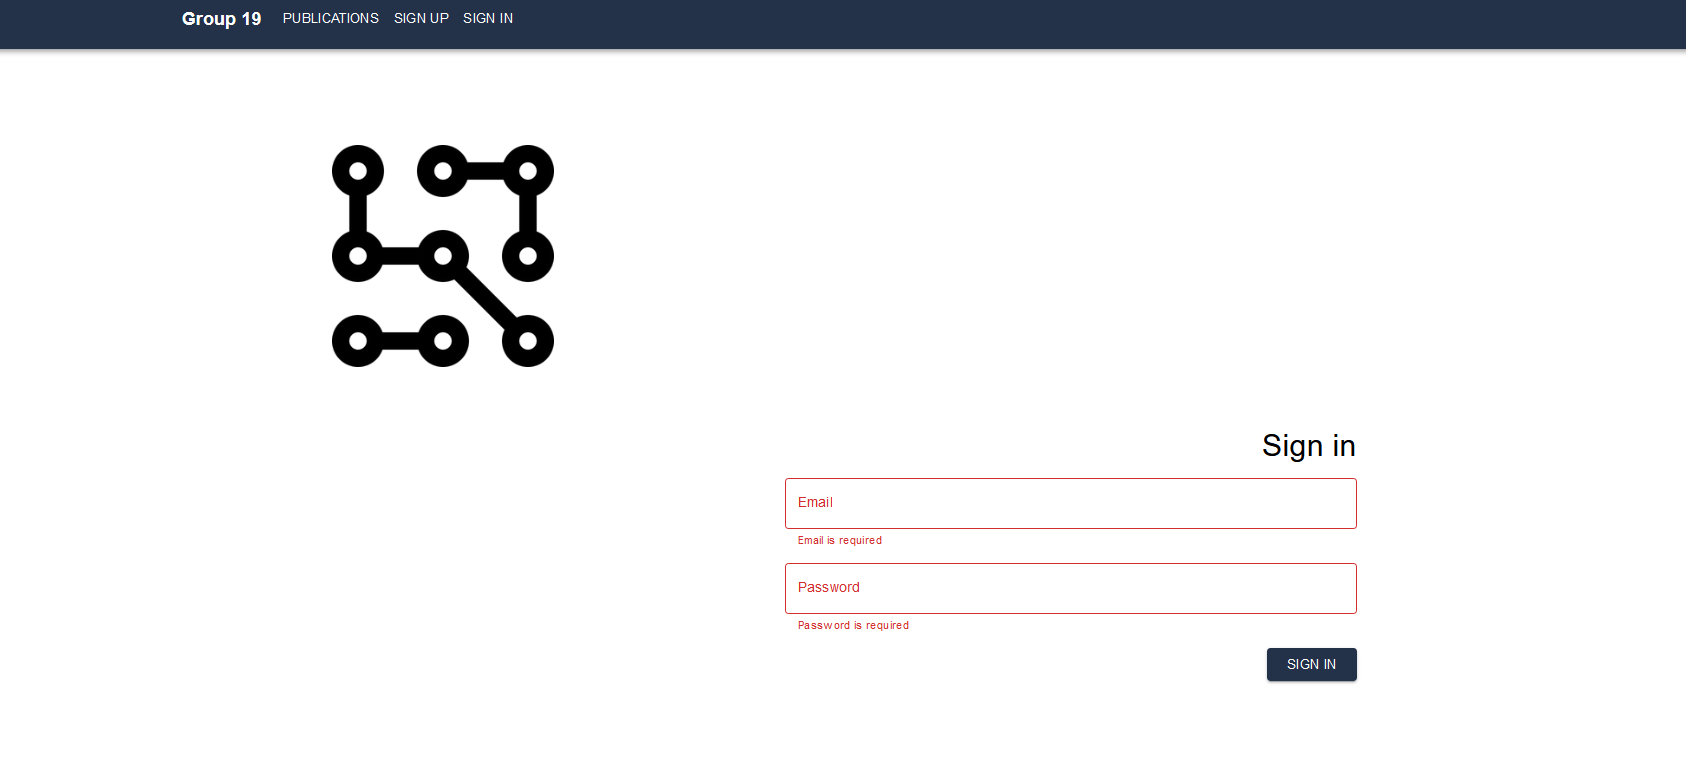
\includegraphics[width=\textwidth]{Picture12}
	\caption{Values are missing and need to be entered}
\end{figure}

\newpage
\subsection{Invalid Email}
This occurs when the email entered is not a valid email. This can be fixed by ensuring the information inputted is correct.

\begin{figure}[h]
	\centering
	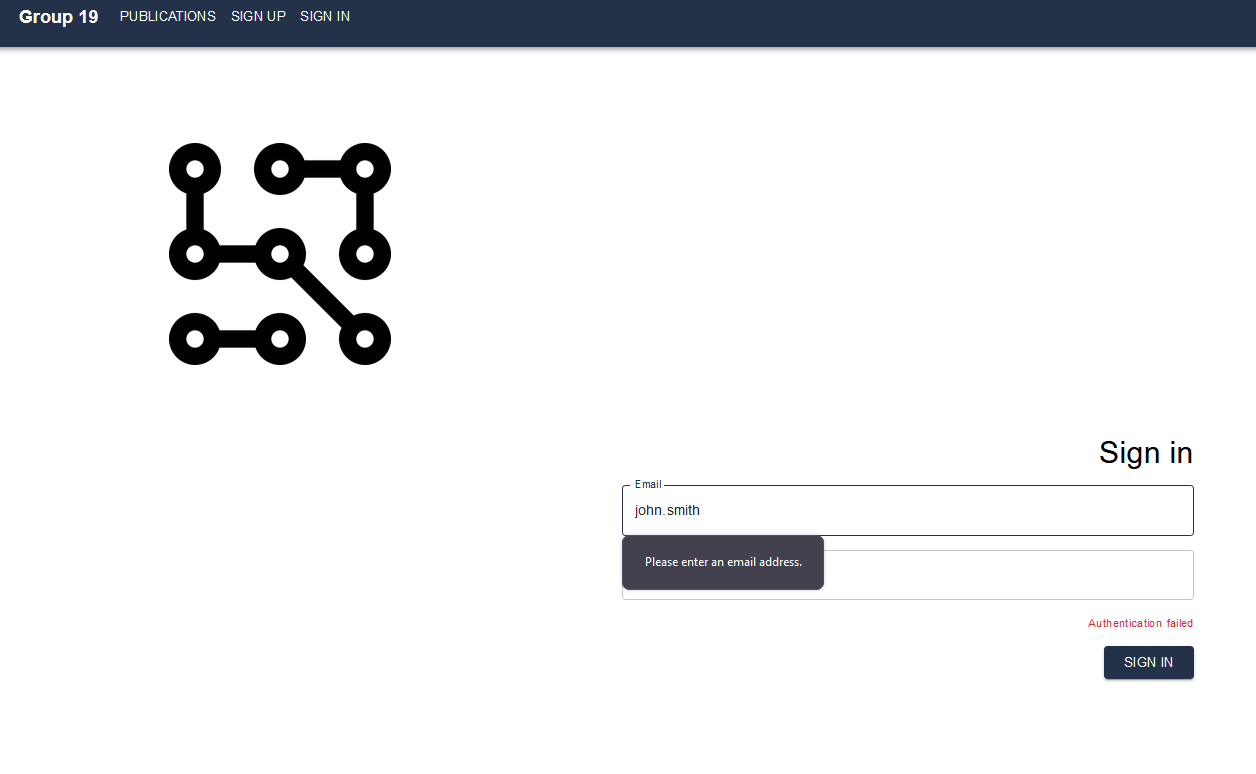
\includegraphics[width=\textwidth]{Picture13}
	\caption{The email entered is not a valid email and needs changing}
\end{figure}

\newpage
\subsection{Authentication Failed}
This occurs when the email and password are not found in the user database. This is most likely caused by incorrect information being inputted

\begin{figure}[h]
	\centering
	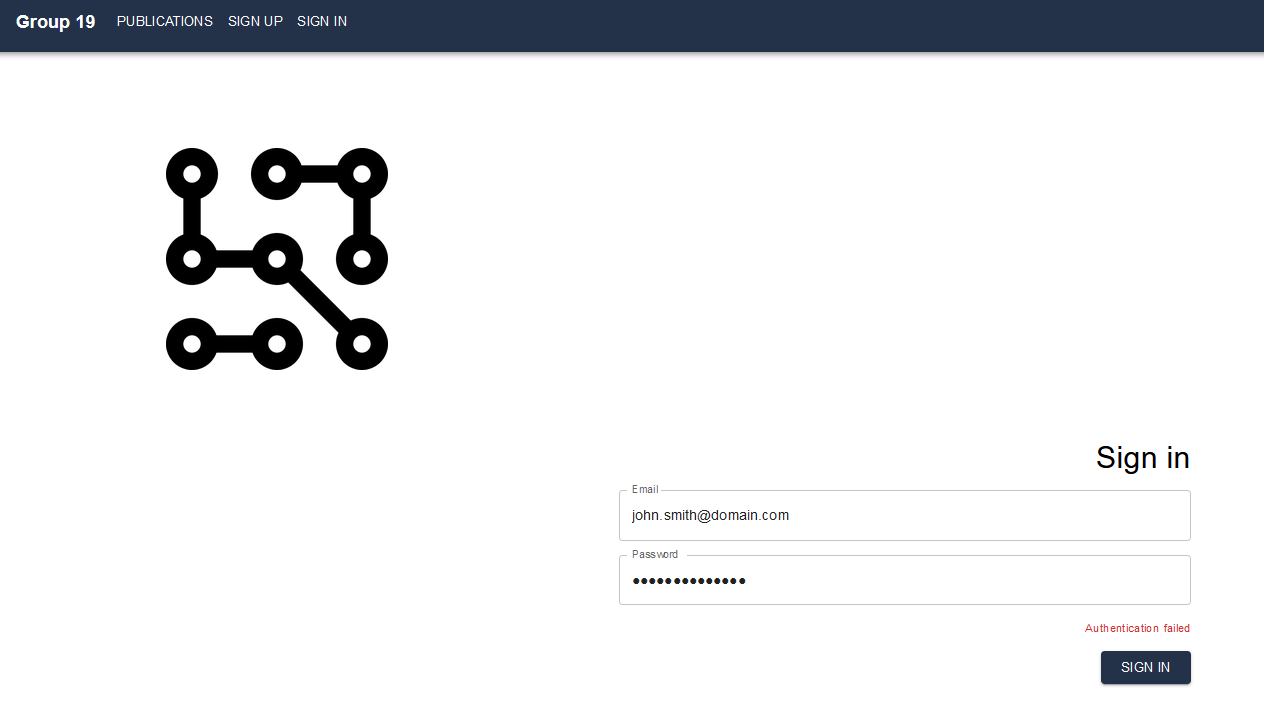
\includegraphics[width=\textwidth]{Picture14}
	\caption{Details inputted are not valid credentials}
\end{figure}

\newpage
\chapter{Account Page}

The account page allows the user to access information about their account. At the top of the page is the email that is assoicated with their account. Below that the user can see their publications and events. These columns also give the user direct access to the edit and delete functions for both publications and events.

\begin{itemize}
	\item \hyperlink{postEdit}{Editing a publication}
	\item \hyperlink{postDelete}{Deleting a publication}
	\item \hyperlink{eventEdit}{Editing an event}
	\item \hyperlink{eventDelete}{Deleting an event}
\end{itemize}

\begin{figure}[h]
	\centering
	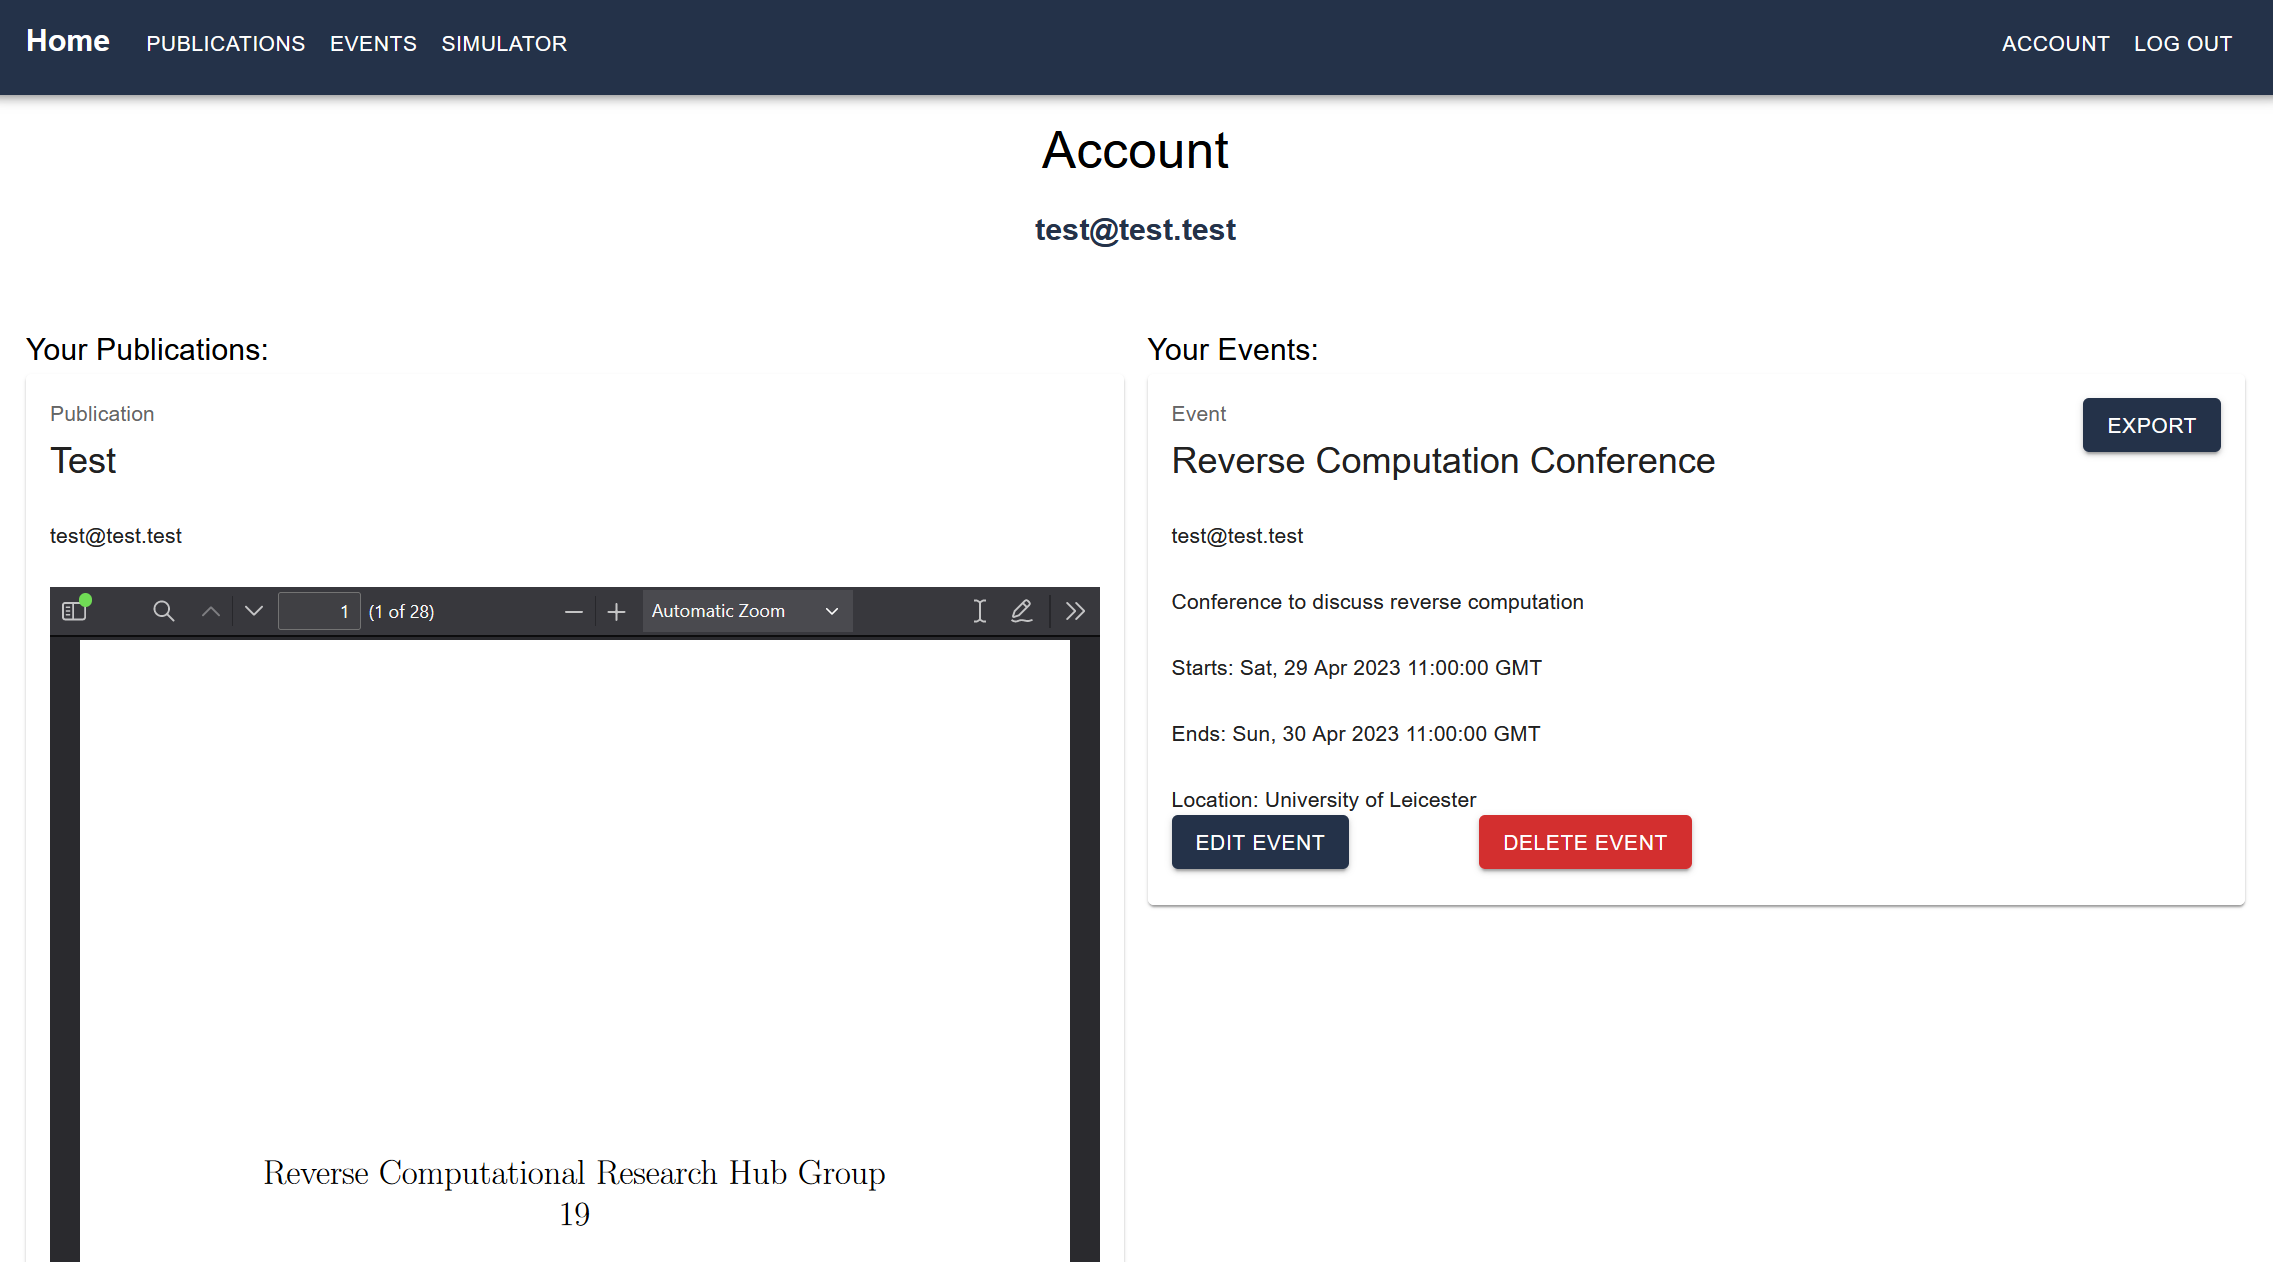
\includegraphics[width=\textwidth]{AccountPage}
	\caption{Account page displaying account details and posts}
\end{figure}



\newpage
\chapter{Publications}

From the homepage, the user can click ‘Publications’ to be navigated to this section.
Here they will see other publication posts with embedded pdfs ordered chronologically along with functionality to create their own publication. A title and a description of the publication is visible.

\begin{figure}[h]
	\centering
	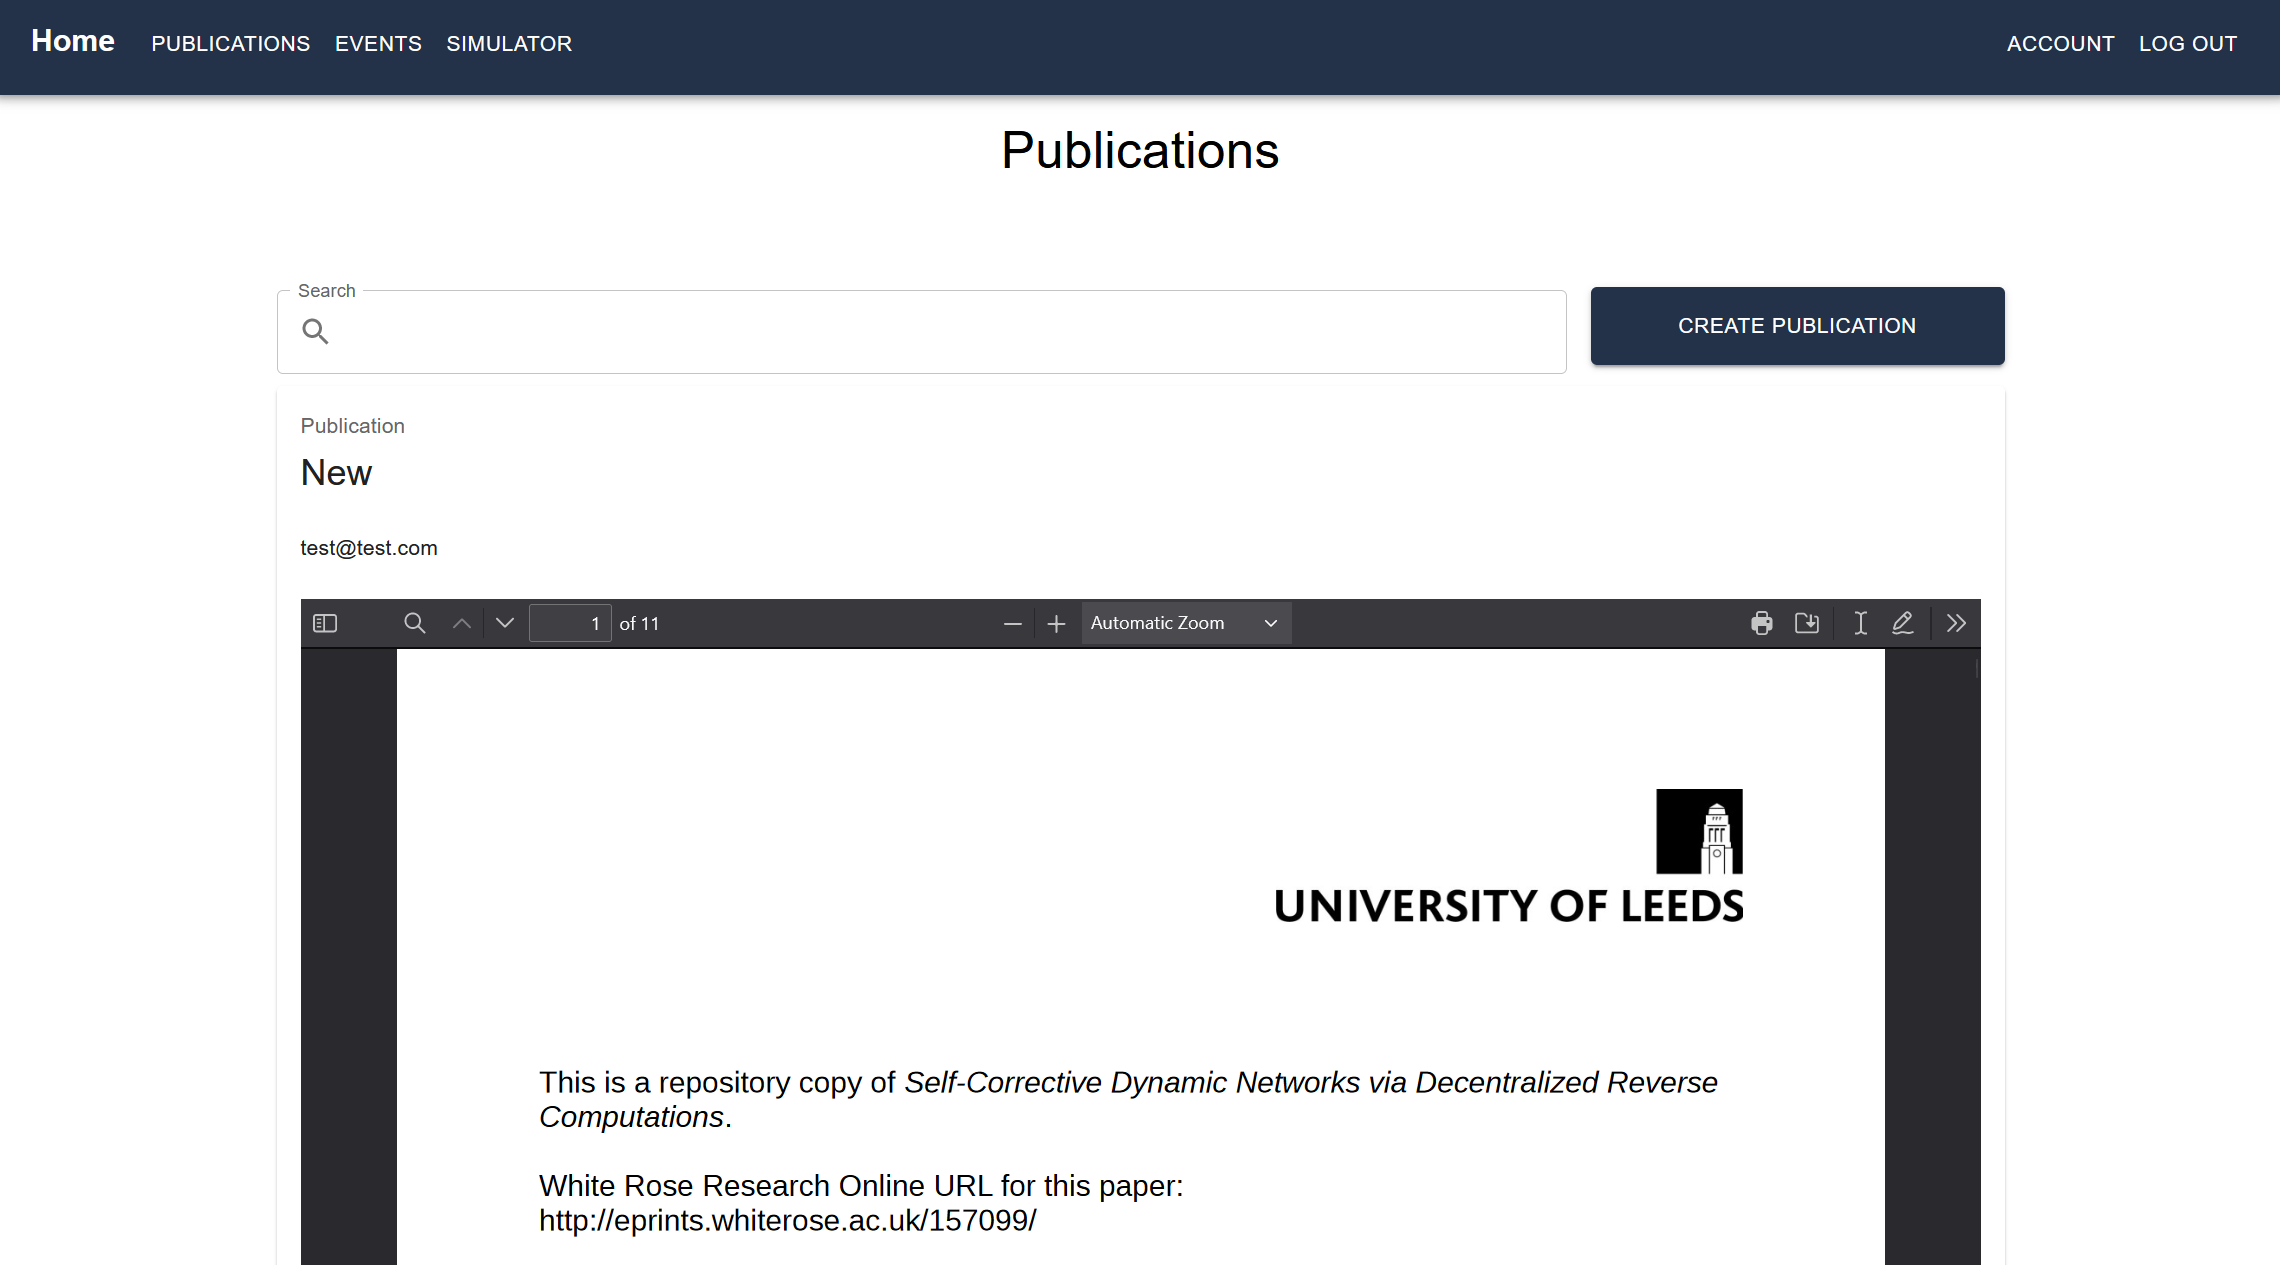
\includegraphics[width=\textwidth]{PublicationPage}
	\caption{Publication page}
\end{figure}

\newpage
\section{Creating a Publication}

To create a post, the user can click ‘create publication’. 

\begin{figure}[h]
	\centering
	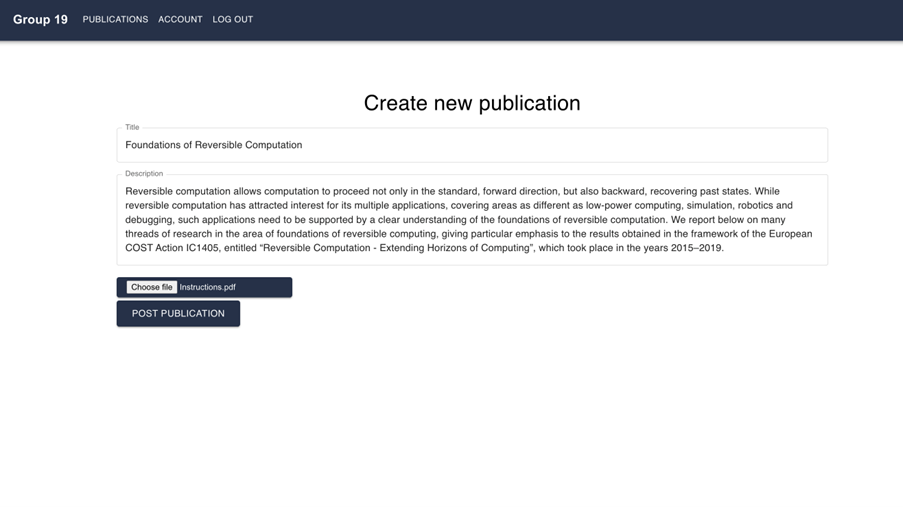
\includegraphics[width=\textwidth]{Picture6}
	\caption{Create New Publication}
\end{figure}

On this page, the user is provided the opportunity to add a title, description, and a pdf. To upload the pdf, click ‘Choose File’, which will then open the operating system file selector. The user can then click ‘Post Publication’ which then uploads the post to the site. It can then be viewed on the publications page

\newpage
\section{Searching for a Publication}

At the top of the publications page, the user can search for specific documents. This can be done by entering keywords into the searchbar. The webpage will then update to only show posts that include the keyword.

\begin{figure}[h]
	\centering
	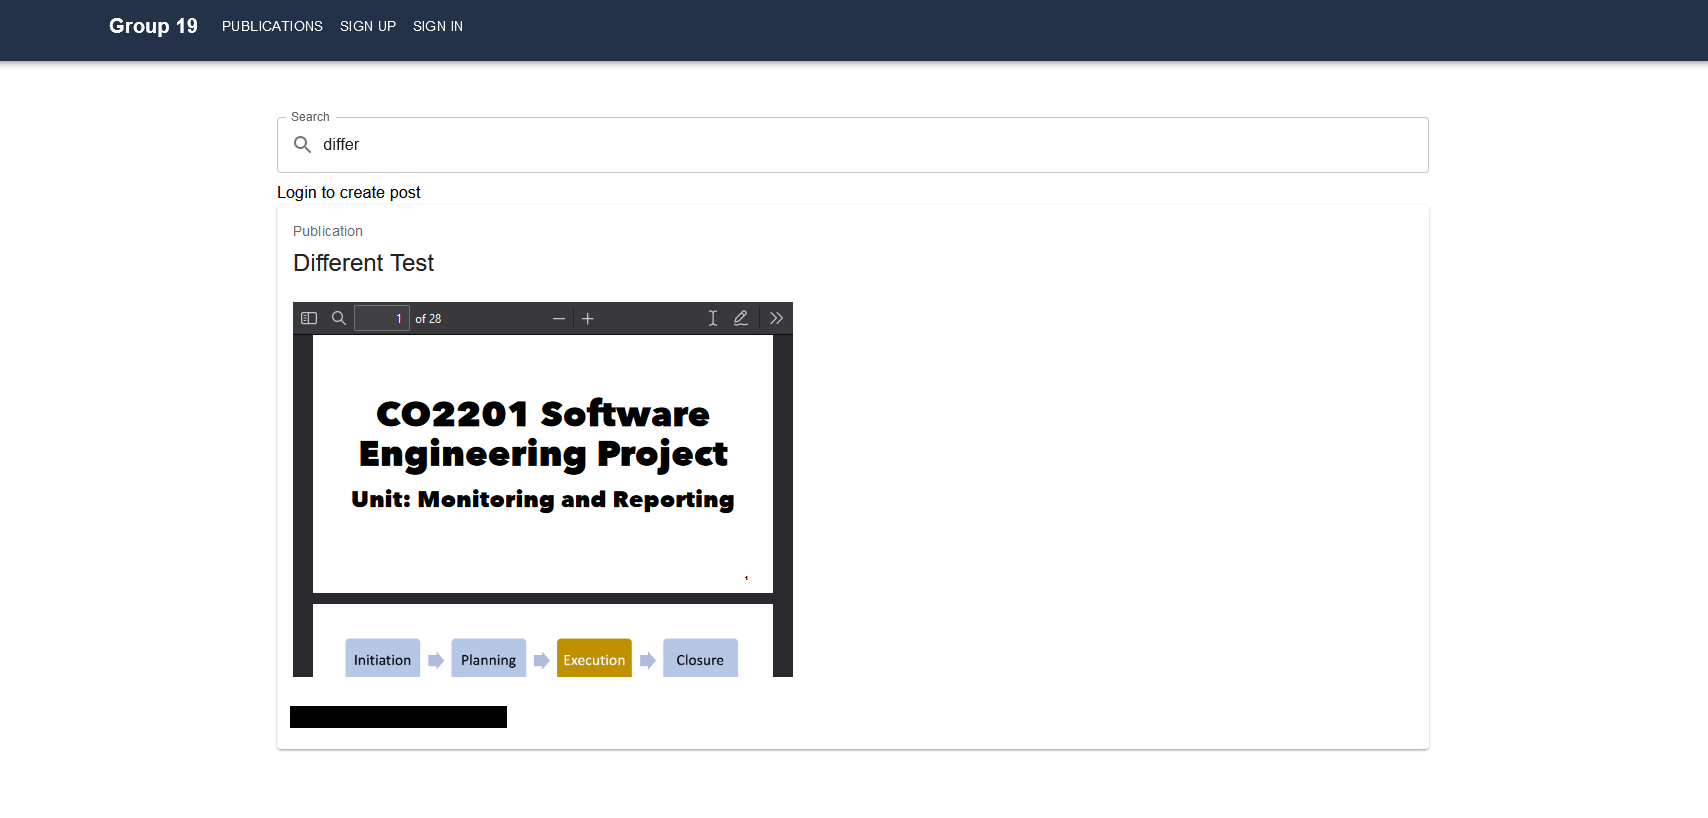
\includegraphics[width=\textwidth]{Picture8}
	\caption{Searching the publications for a specific post}
\end{figure}

\newpage
\hypertarget{postDelete}{}
\section{Deleting a Publication}


If the user needs to remove a publication for whatever reason, that is also possible. Each post the current user has made has a button which removes the post when clicked.

\begin{figure}[h]t
	\centering
	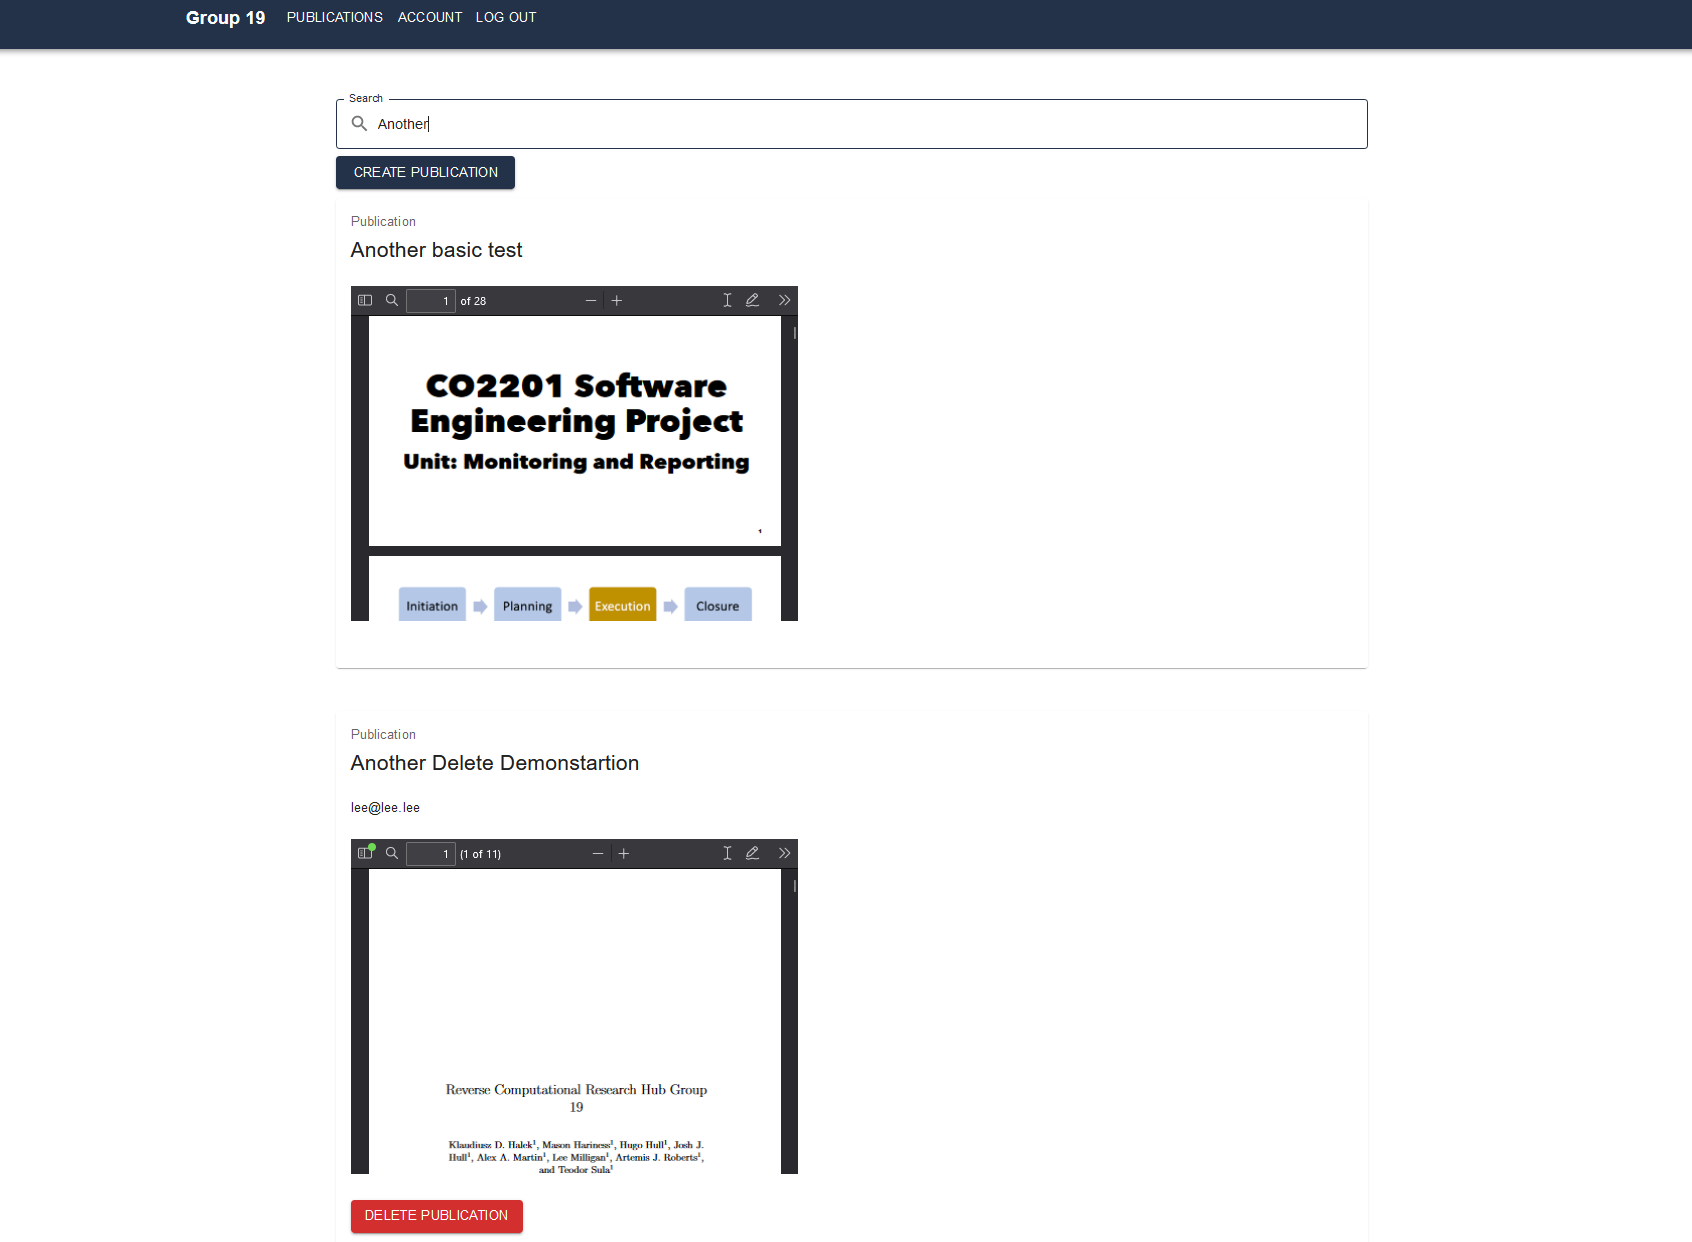
\includegraphics[width=\textwidth]{Picture9}
	\caption{The user can only delete posts they made}
\end{figure}

\begin{figure}[ht]
	\centering
	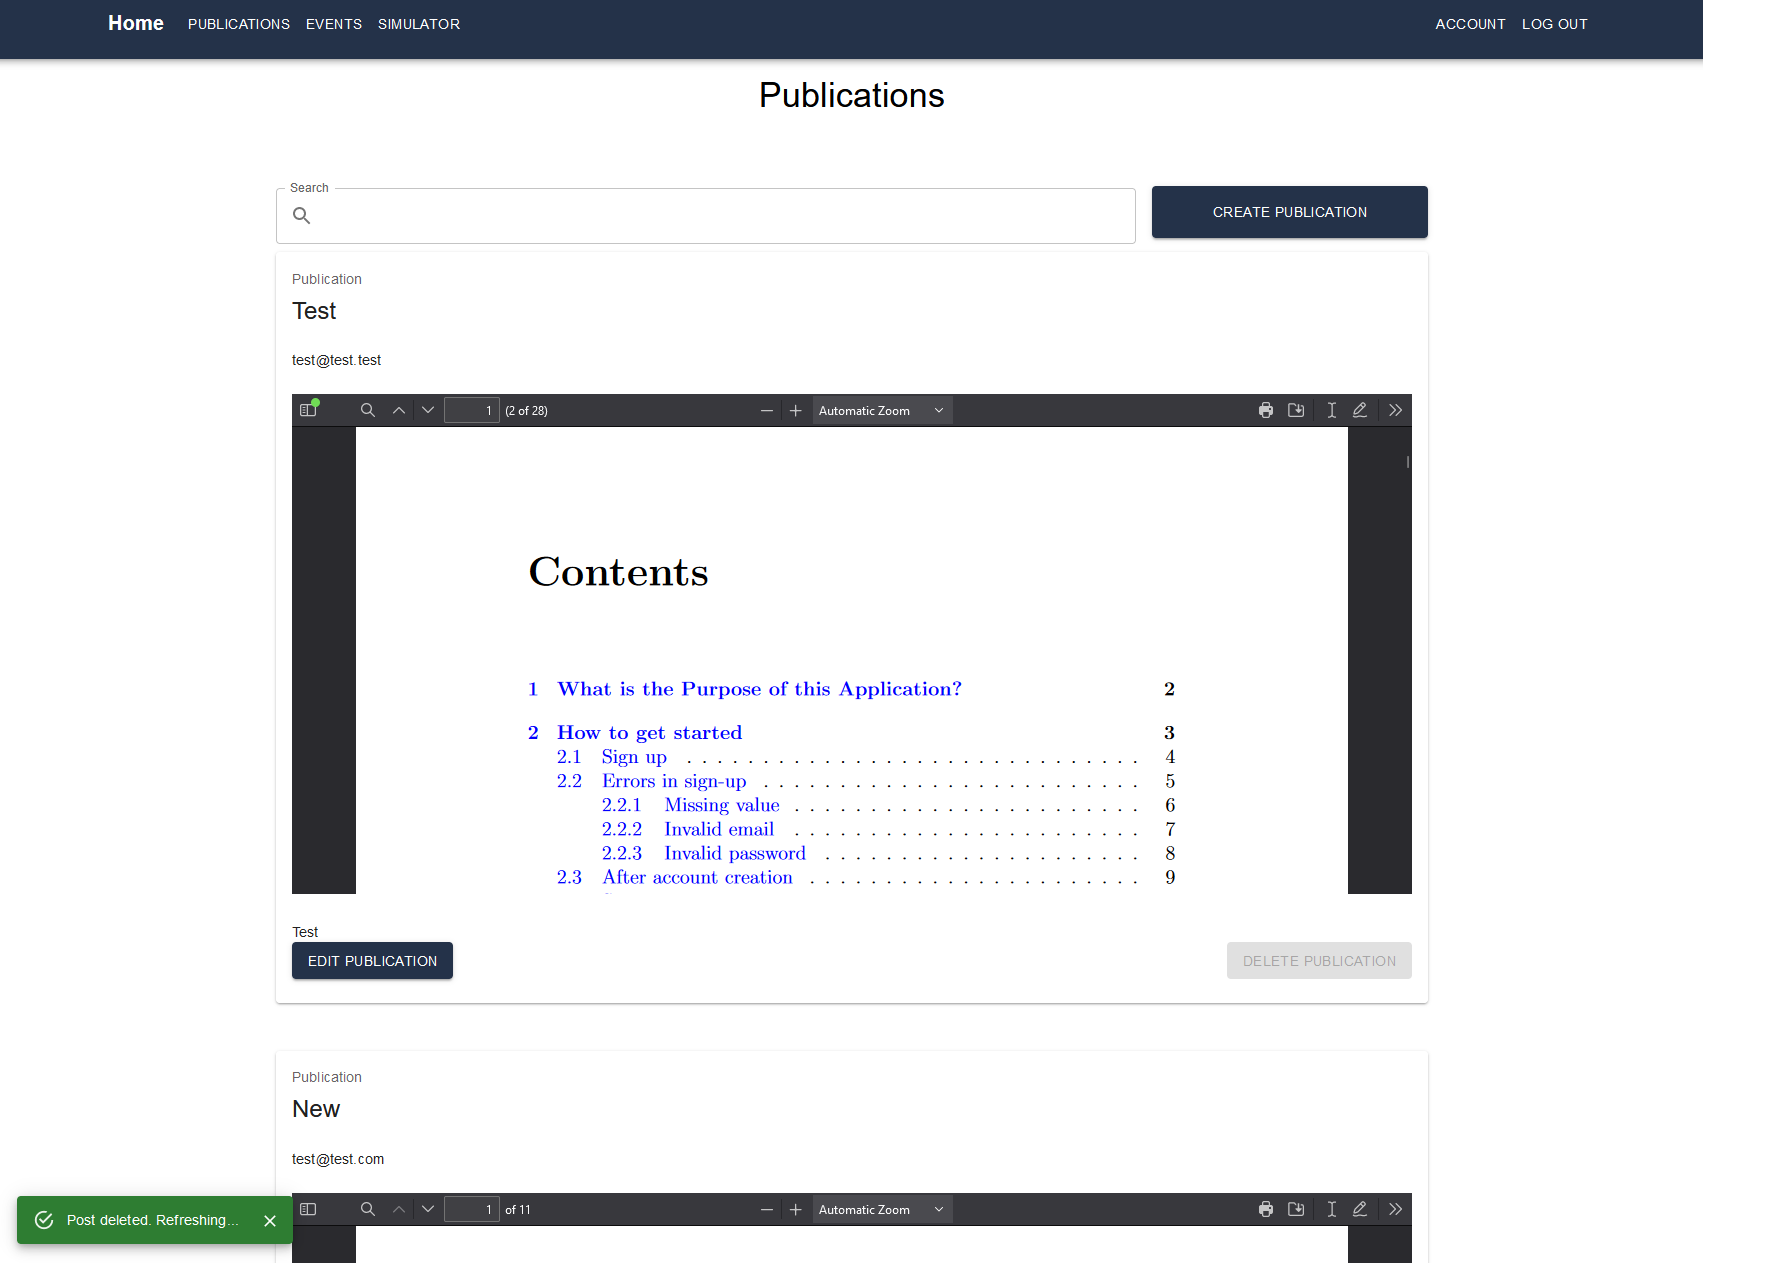
\includegraphics[width=\textwidth]{PublicationPageDelete}
	\caption{The website displays a message to confirm post deletion}
\end{figure}

\begin{figure}[ht]
	\centering
	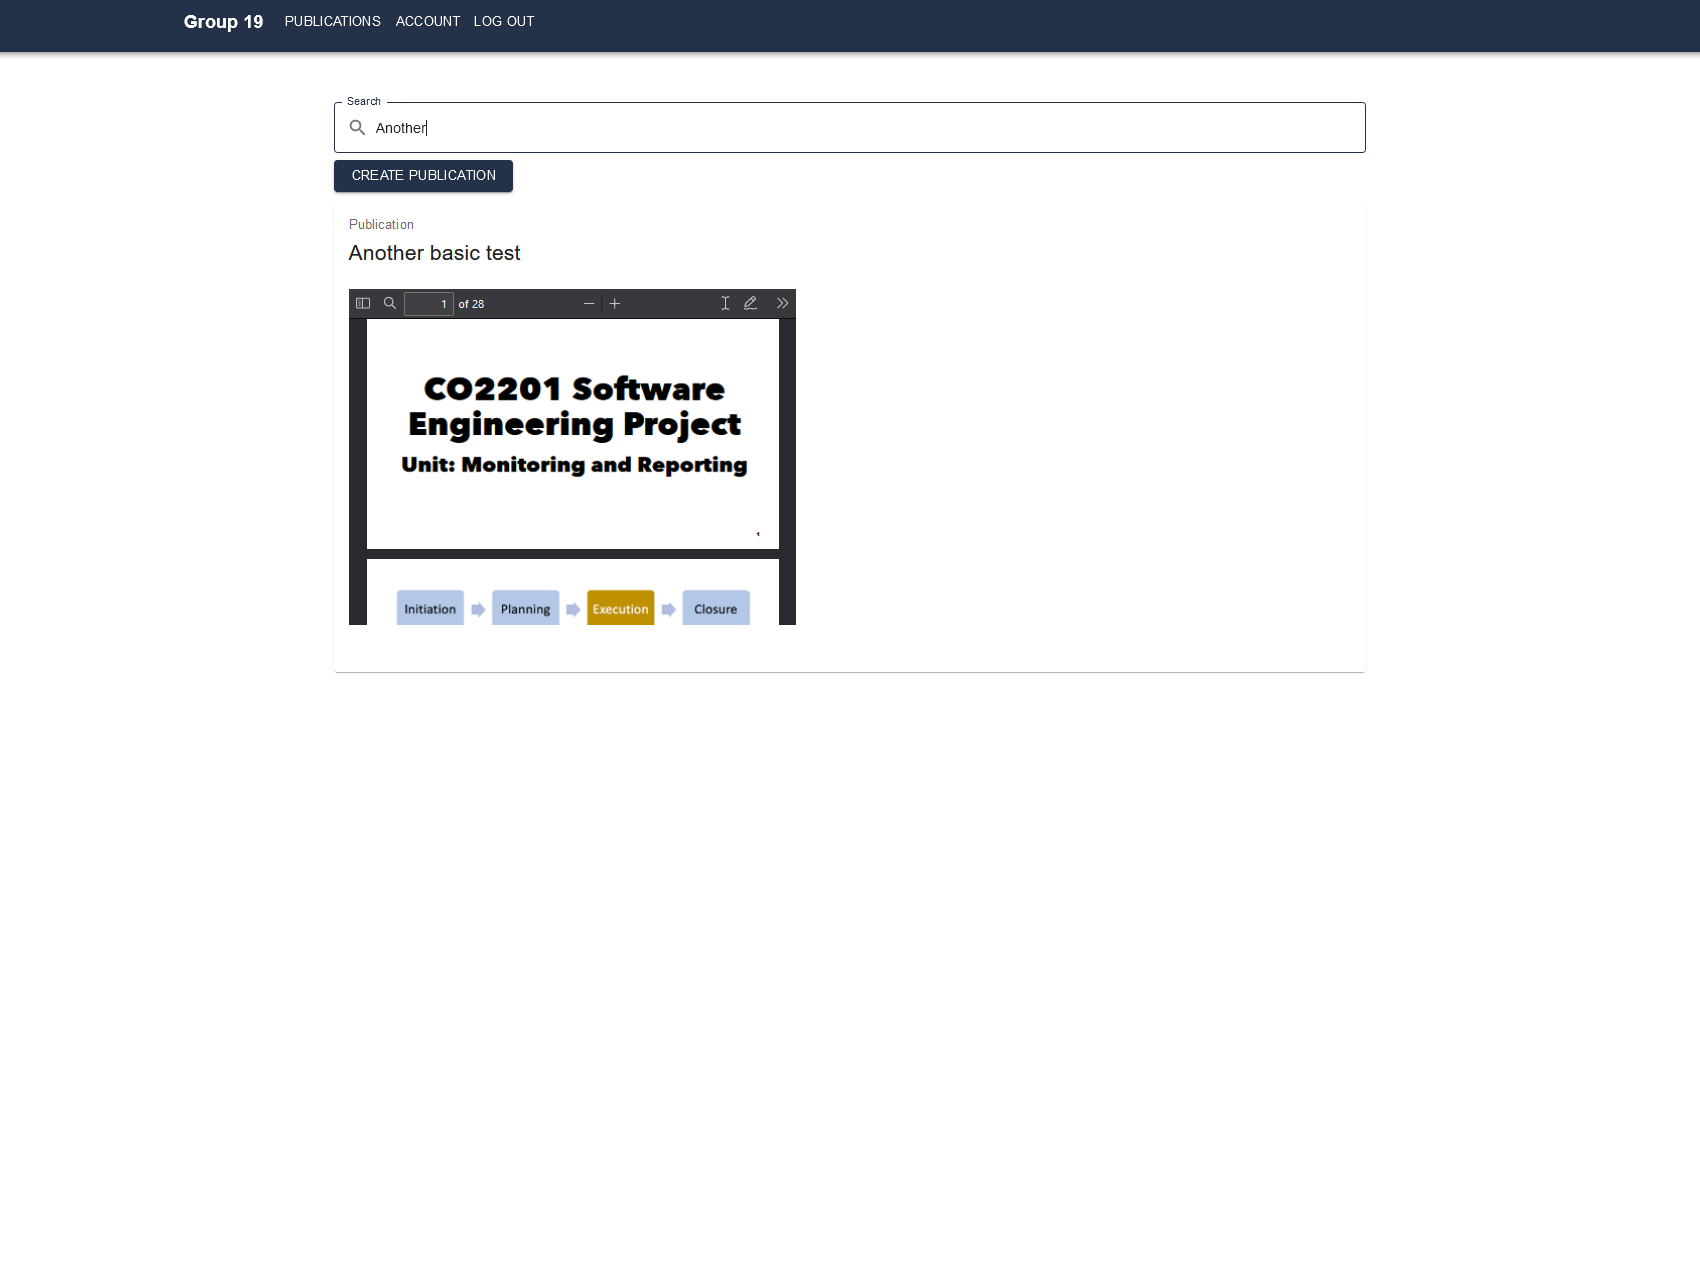
\includegraphics[width=\textwidth]{Picture11}
	\caption{The post is no longer found in the page of posts}
\end{figure}

\FloatBarrier
\hypertarget{postEdit}{}
\section{Editing a Publication}

If the user has inputted incorrect information, they can do so by editing an exisiting publication. The user can only edit posts they have uploaded. They will only be able to change the title and description of an existing post. If they need to update the uploaded file, they will need to \hyperlink{postDelete}{delete the post} and reupload with the correct file.

\begin{figure}[ht]
	\centering
	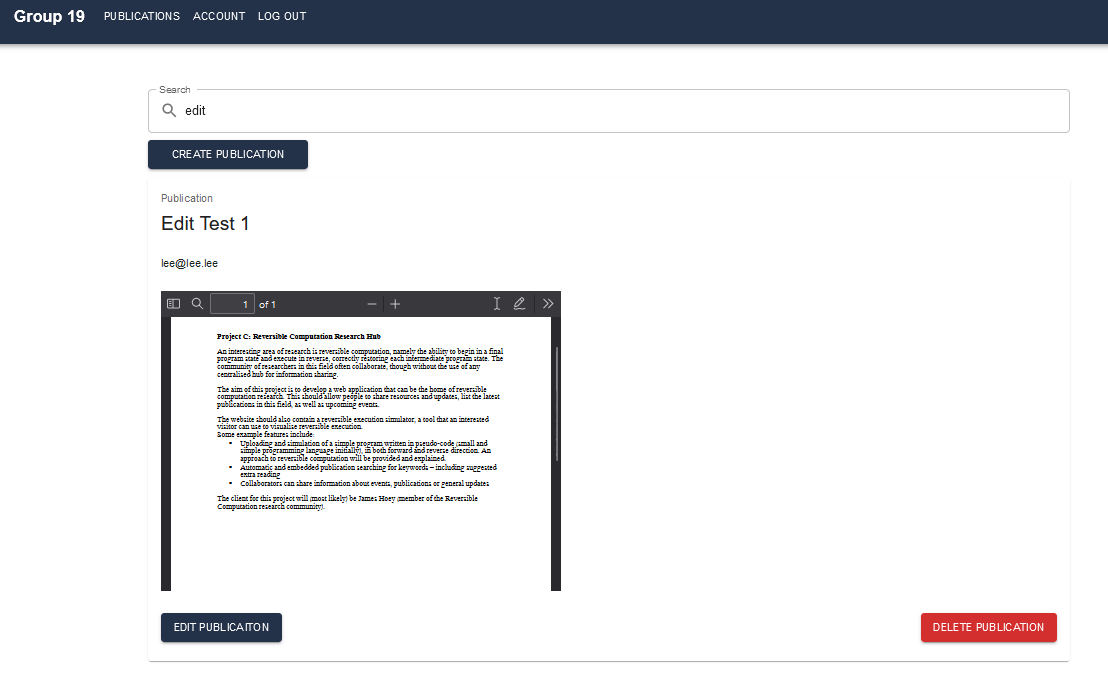
\includegraphics[width=\textwidth]{Picture18}
	\caption{Posts you have created have the option to have details about them editied}
\end{figure}

\begin{figure}[ht]
	\centering
	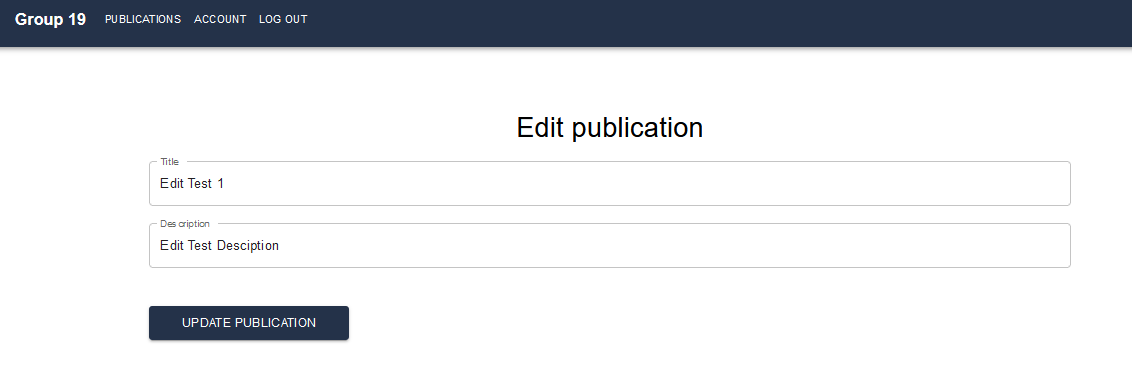
\includegraphics[width=\textwidth]{Picture19}
	\caption{Fields to edit the title and description}
\end{figure}

\begin{figure}[ht]
	\centering
	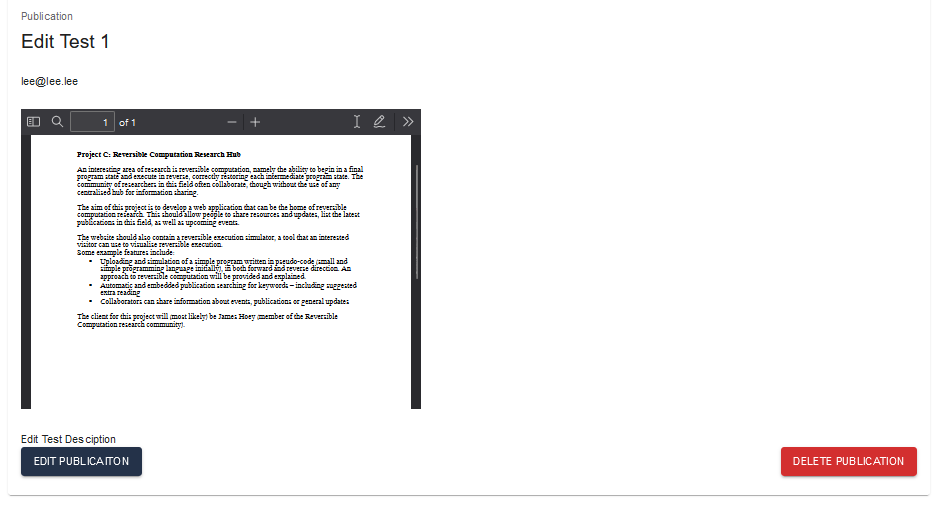
\includegraphics[width=\textwidth]{Picture20}
	\caption{Existing post with new information}
\end{figure}

\newpage
\chapter{Events}

The events page allows users on the website to creating posts with details to real world or online events which other users can then attend. This is helpful to inform the community of conferences and meetups that may be of relevance to them. There is also an area to write out details of the event to get more information across.

\begin{figure}[ht]
	\centering
	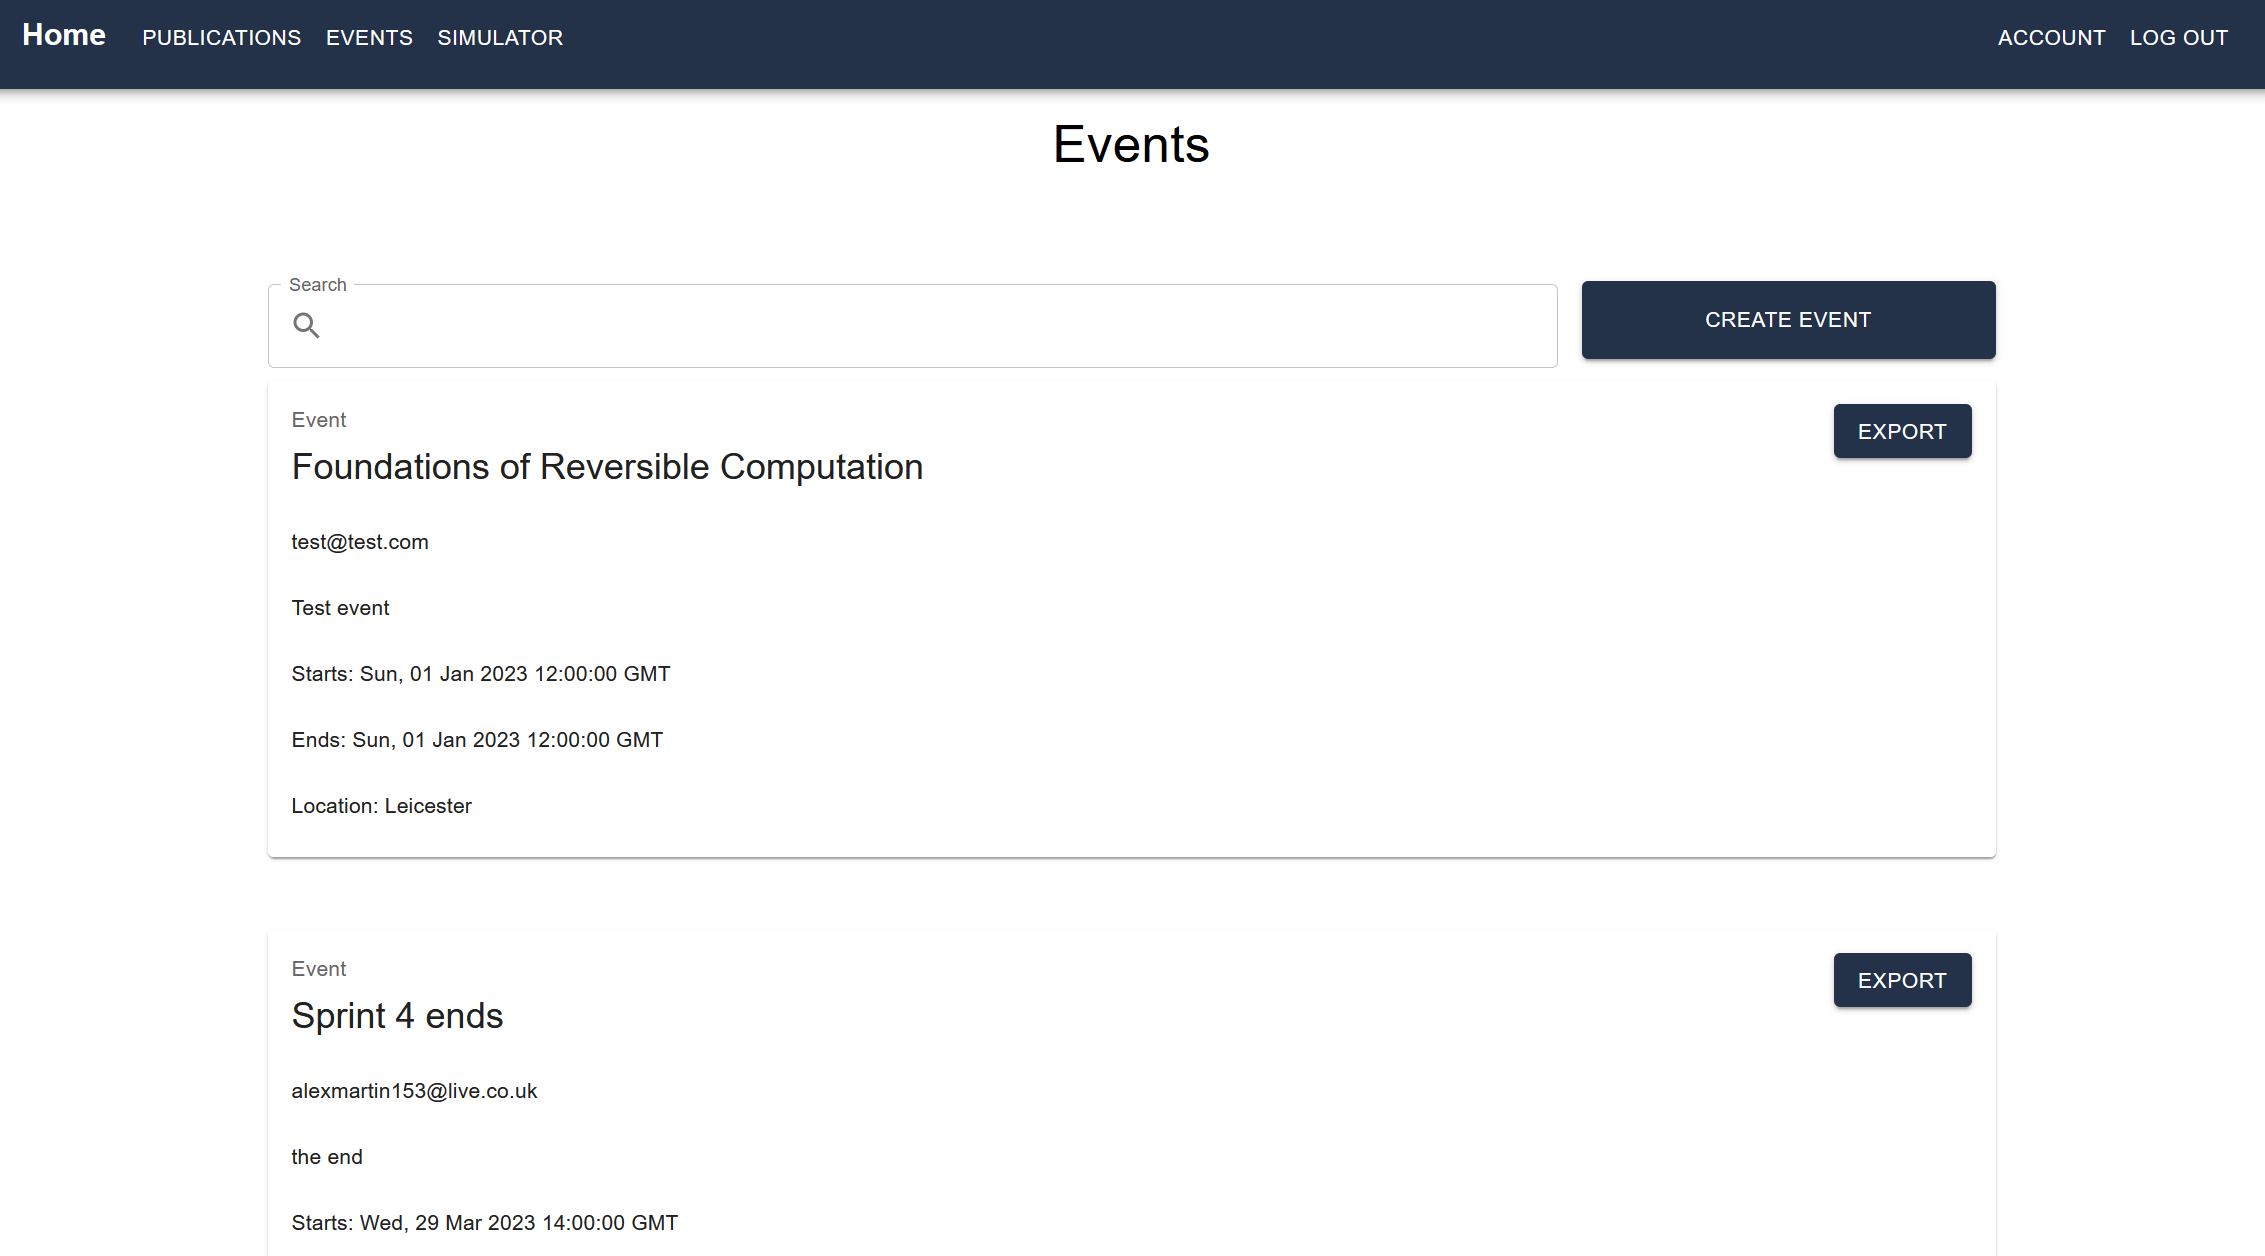
\includegraphics[width=\textwidth]{EventPage}
	\caption{Example event page with events listed}
\end{figure}

\section{Creating an Event}

A logged-in user can create an event by clicking on the 'Create Event' button which can be found next to the event search bar on the main event page. If the user is not logged-in there will be a prompt to login.

\begin{figure}[ht]
	\centering
	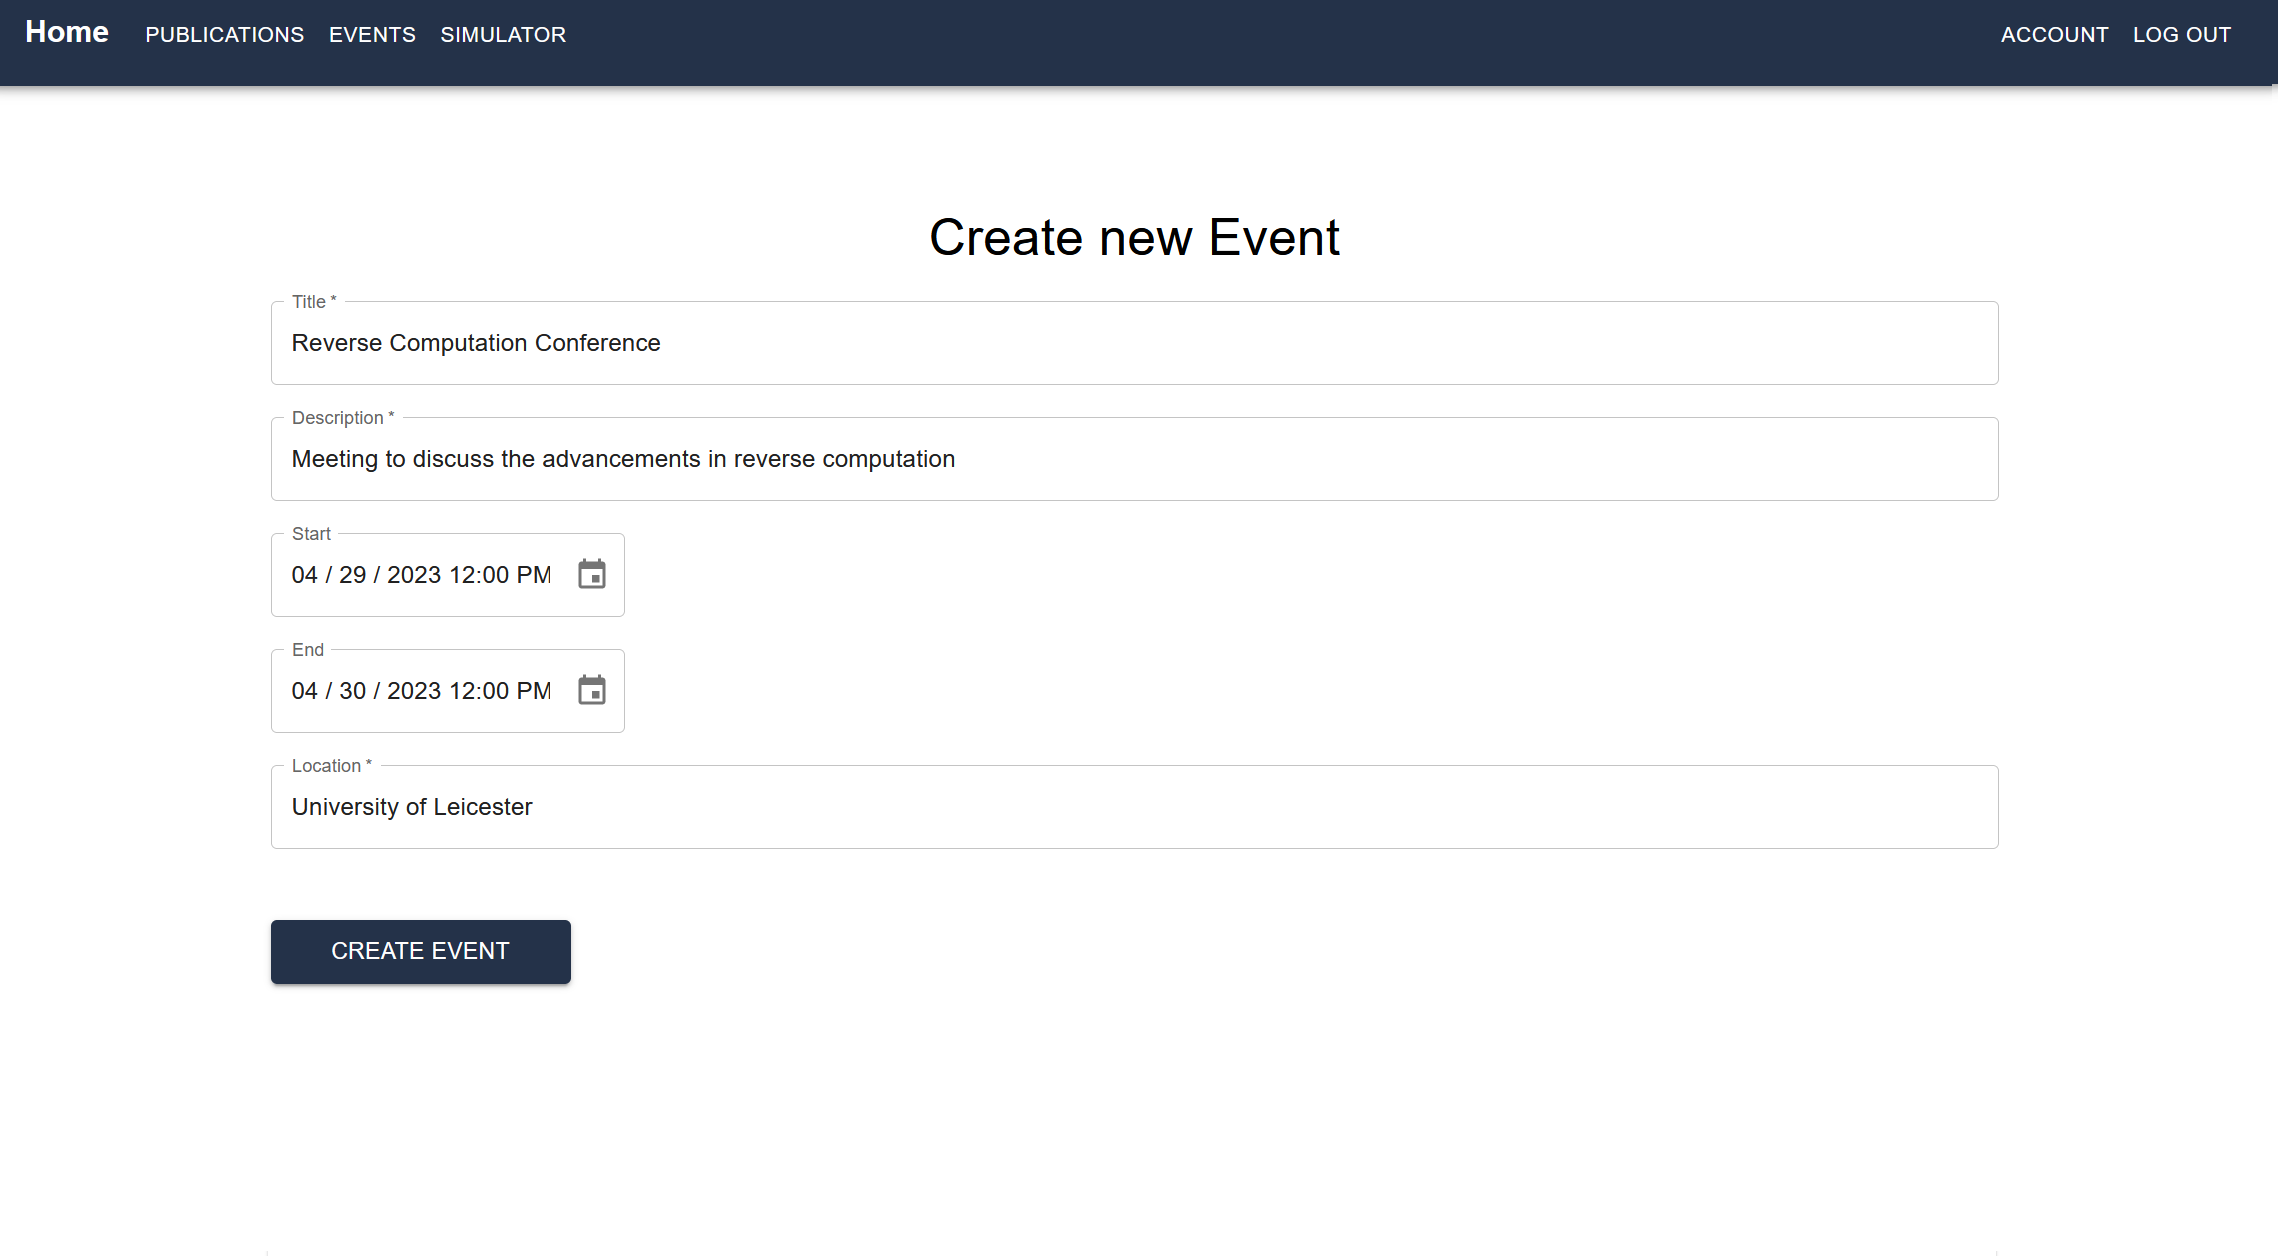
\includegraphics[width=\textwidth]{EventPageCreation}
	\caption{Event Creation Page}
\end{figure}

On the event creation page, there are fields to add: Title, Description, Start time, end time and Location. If the user has made a mistake or need to update the information they originally inputted, they can do so by \hyperlink{eventEdit}{editing the event}.

\newpage
\section{Searching the Events for a Specific Listing}

At the top of the events page, the user can search for specific events. This can be done by entering keywords into the searchbar. The webpage will then update to only show events that include the keyword.

\begin{figure}[h]
	\centering
	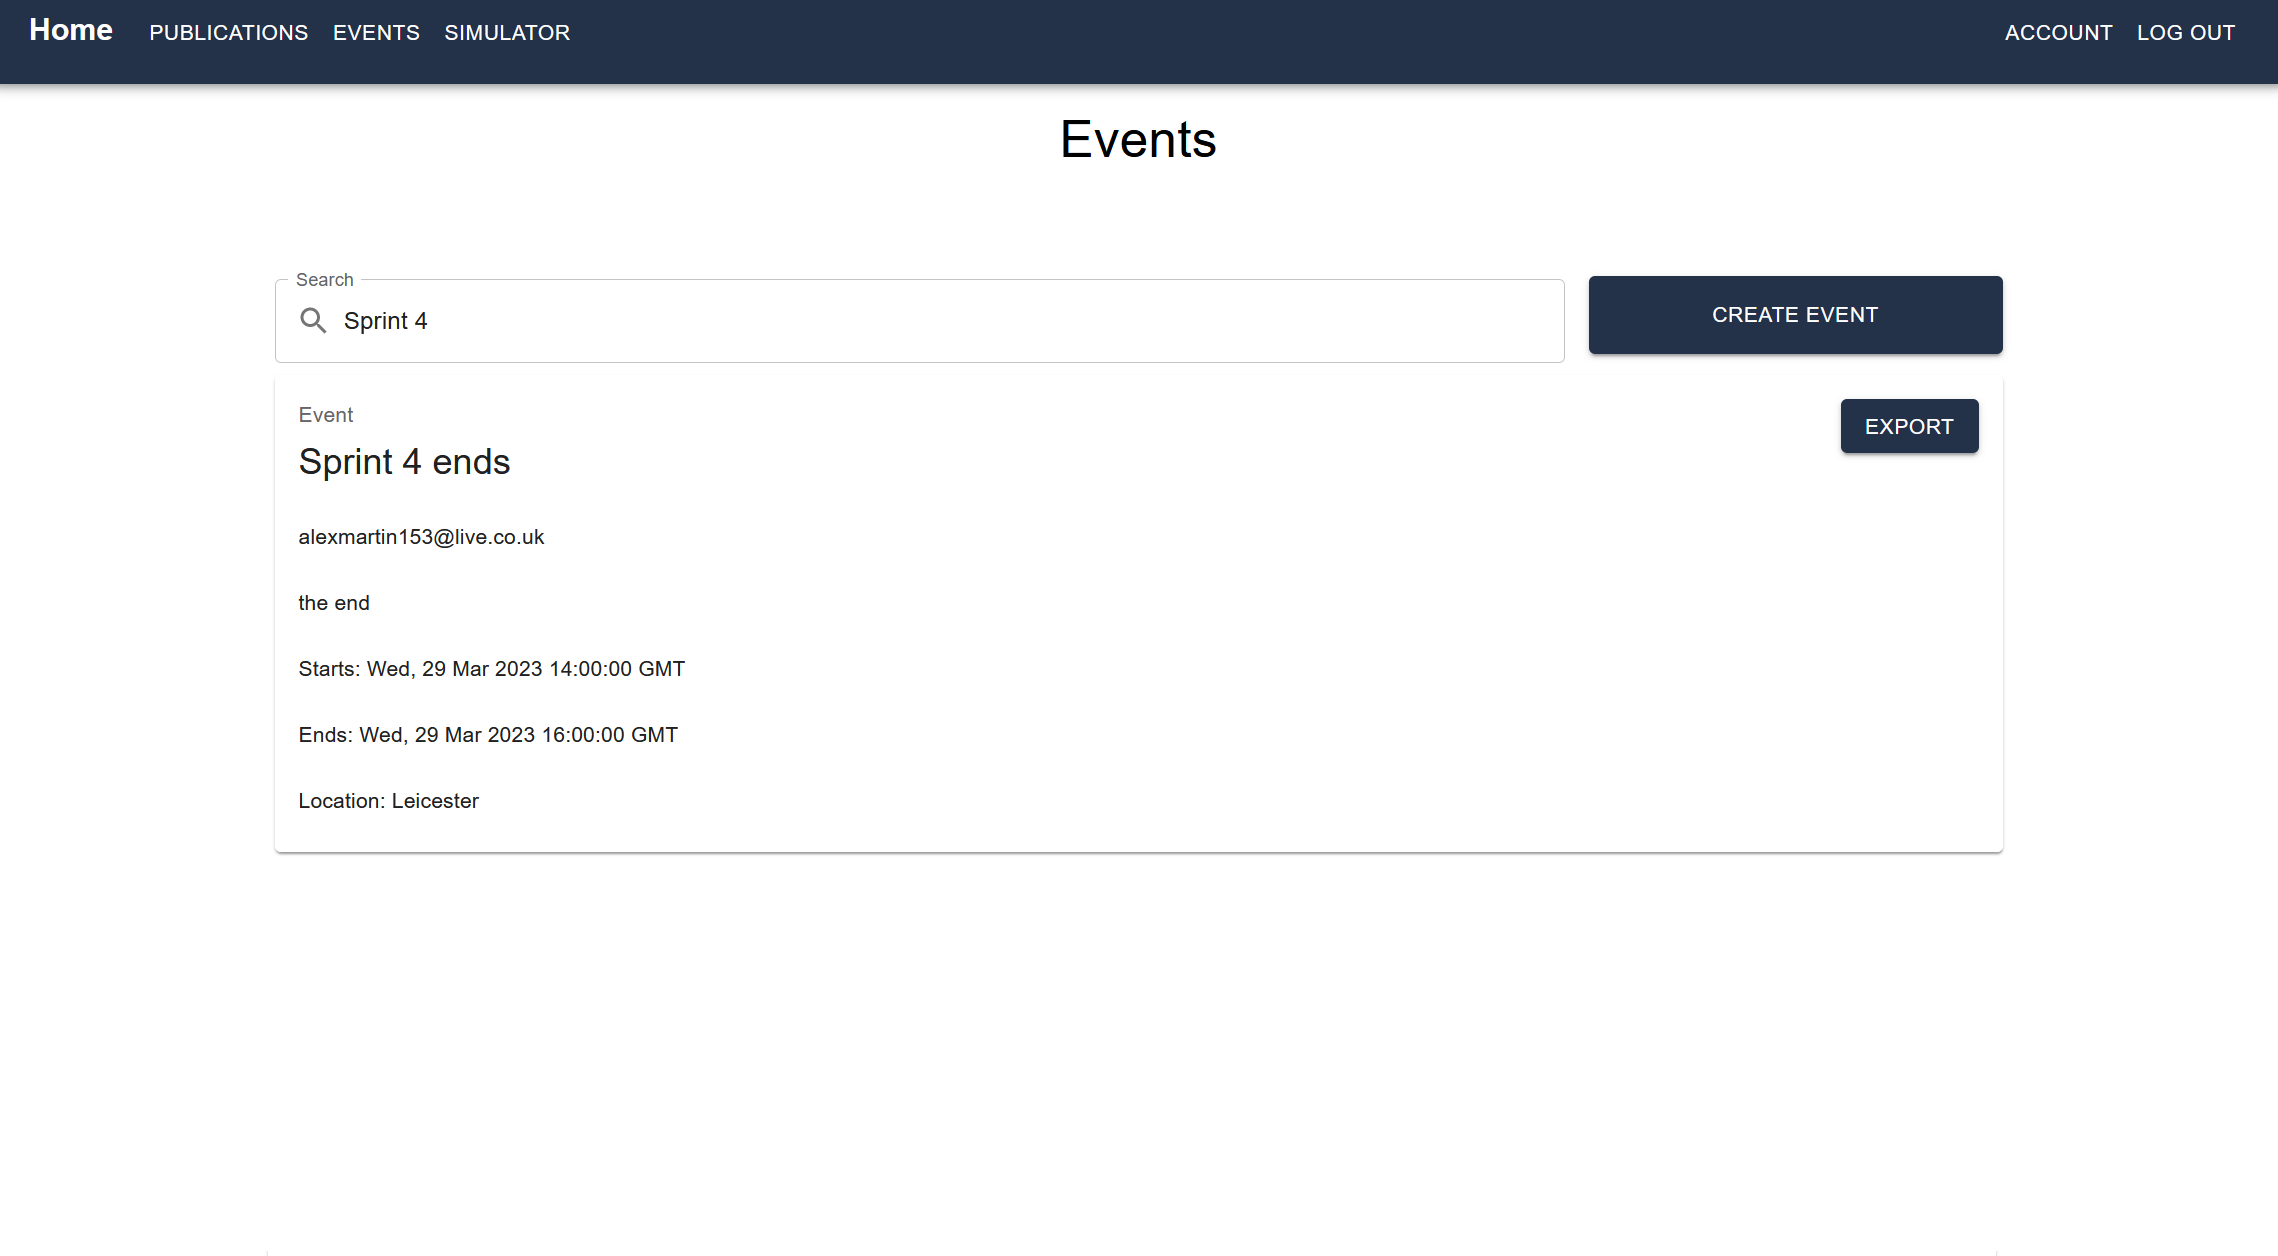
\includegraphics[width=\textwidth]{EventPageSearch}
	\caption{Searching for an event}
\end{figure}

\newpage
\hypertarget{eventDelete}{}
\section{Deleting an Event}

If the user needs to remove an event for whatever reason, that is also possible. Each event the current user has made has a button which removes the post when clicked.

\begin{figure}[h]
	\centering
	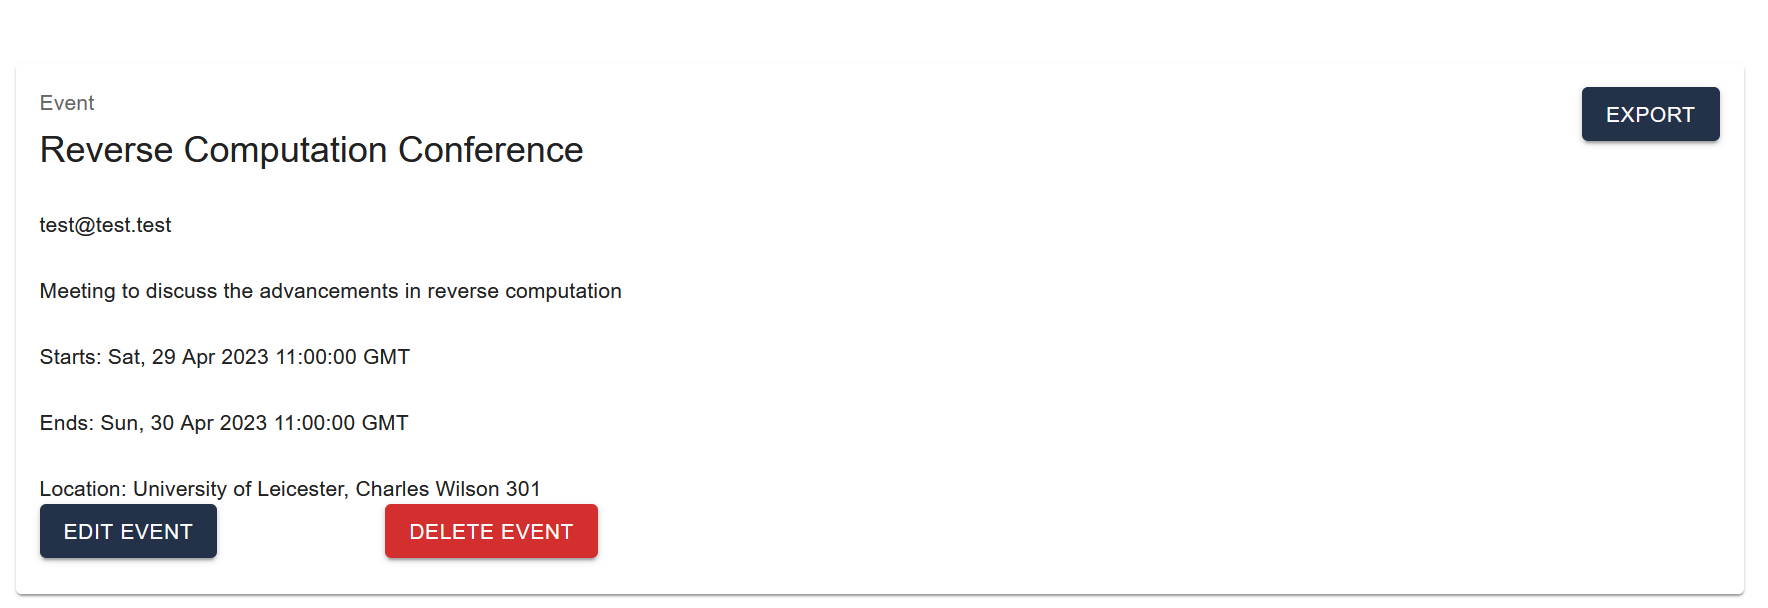
\includegraphics[width=\textwidth]{EventPageEdit3}
	\caption{Button to delete an event the user created}
\end{figure}

\begin{figure}[h]
	\centering
	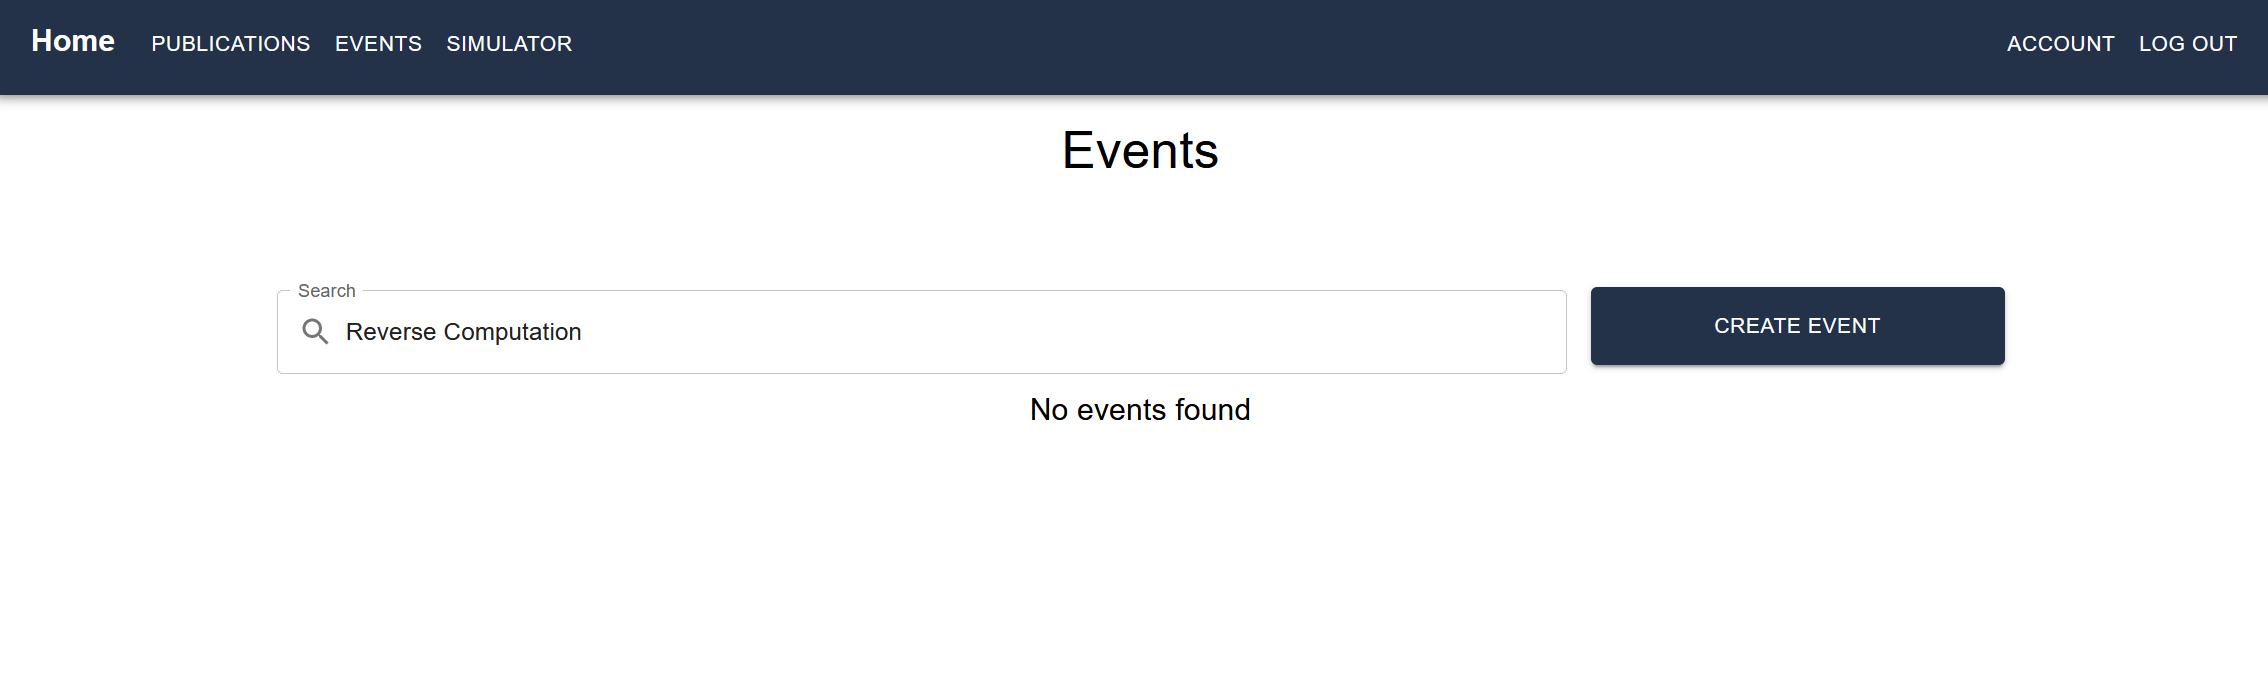
\includegraphics[width=\textwidth]{EventPageDelete2}
	\caption{Event is deleted from website}
\end{figure}

\newpage
\hypertarget{eventEdit}{}
\section{Editing an Event}

You are also able to edit events that you have created. This can be done by navigating to your event and clicking the 'Edit Event' button. This will then bring the user to the edit event page.

\begin{figure}[h]
	\centering
	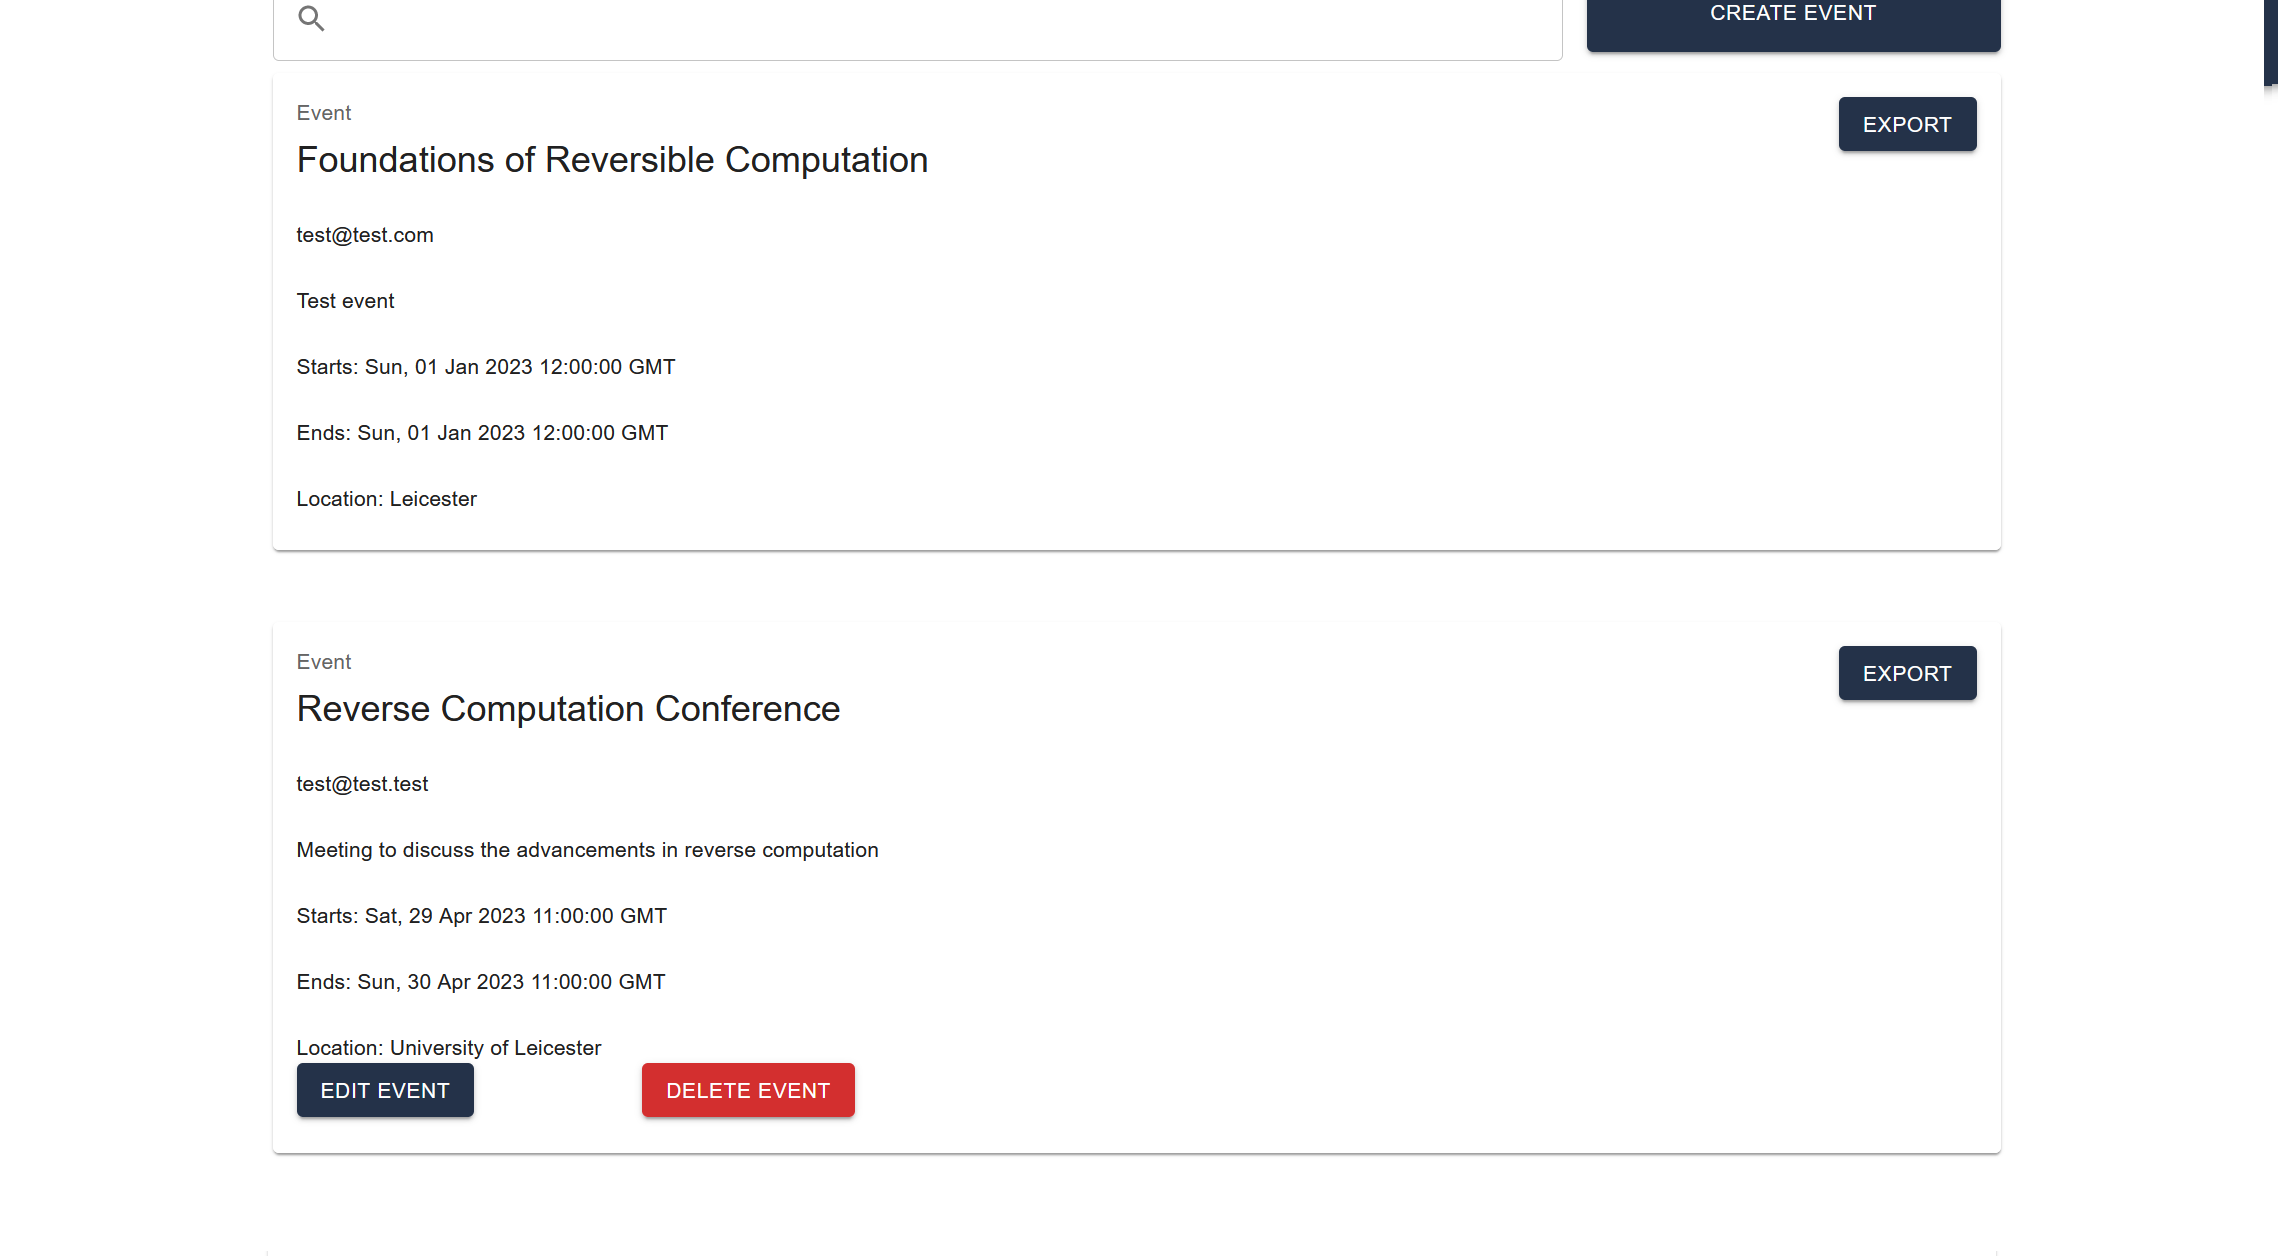
\includegraphics[width=\textwidth]{EventPageEdit1}
	\caption{Event Before Editing}
\end{figure}

On the event edit page, you can update any of the fields with new information and then click the 'Edit Event' button to push these changes to the website

\begin{figure}[h]
	\centering
	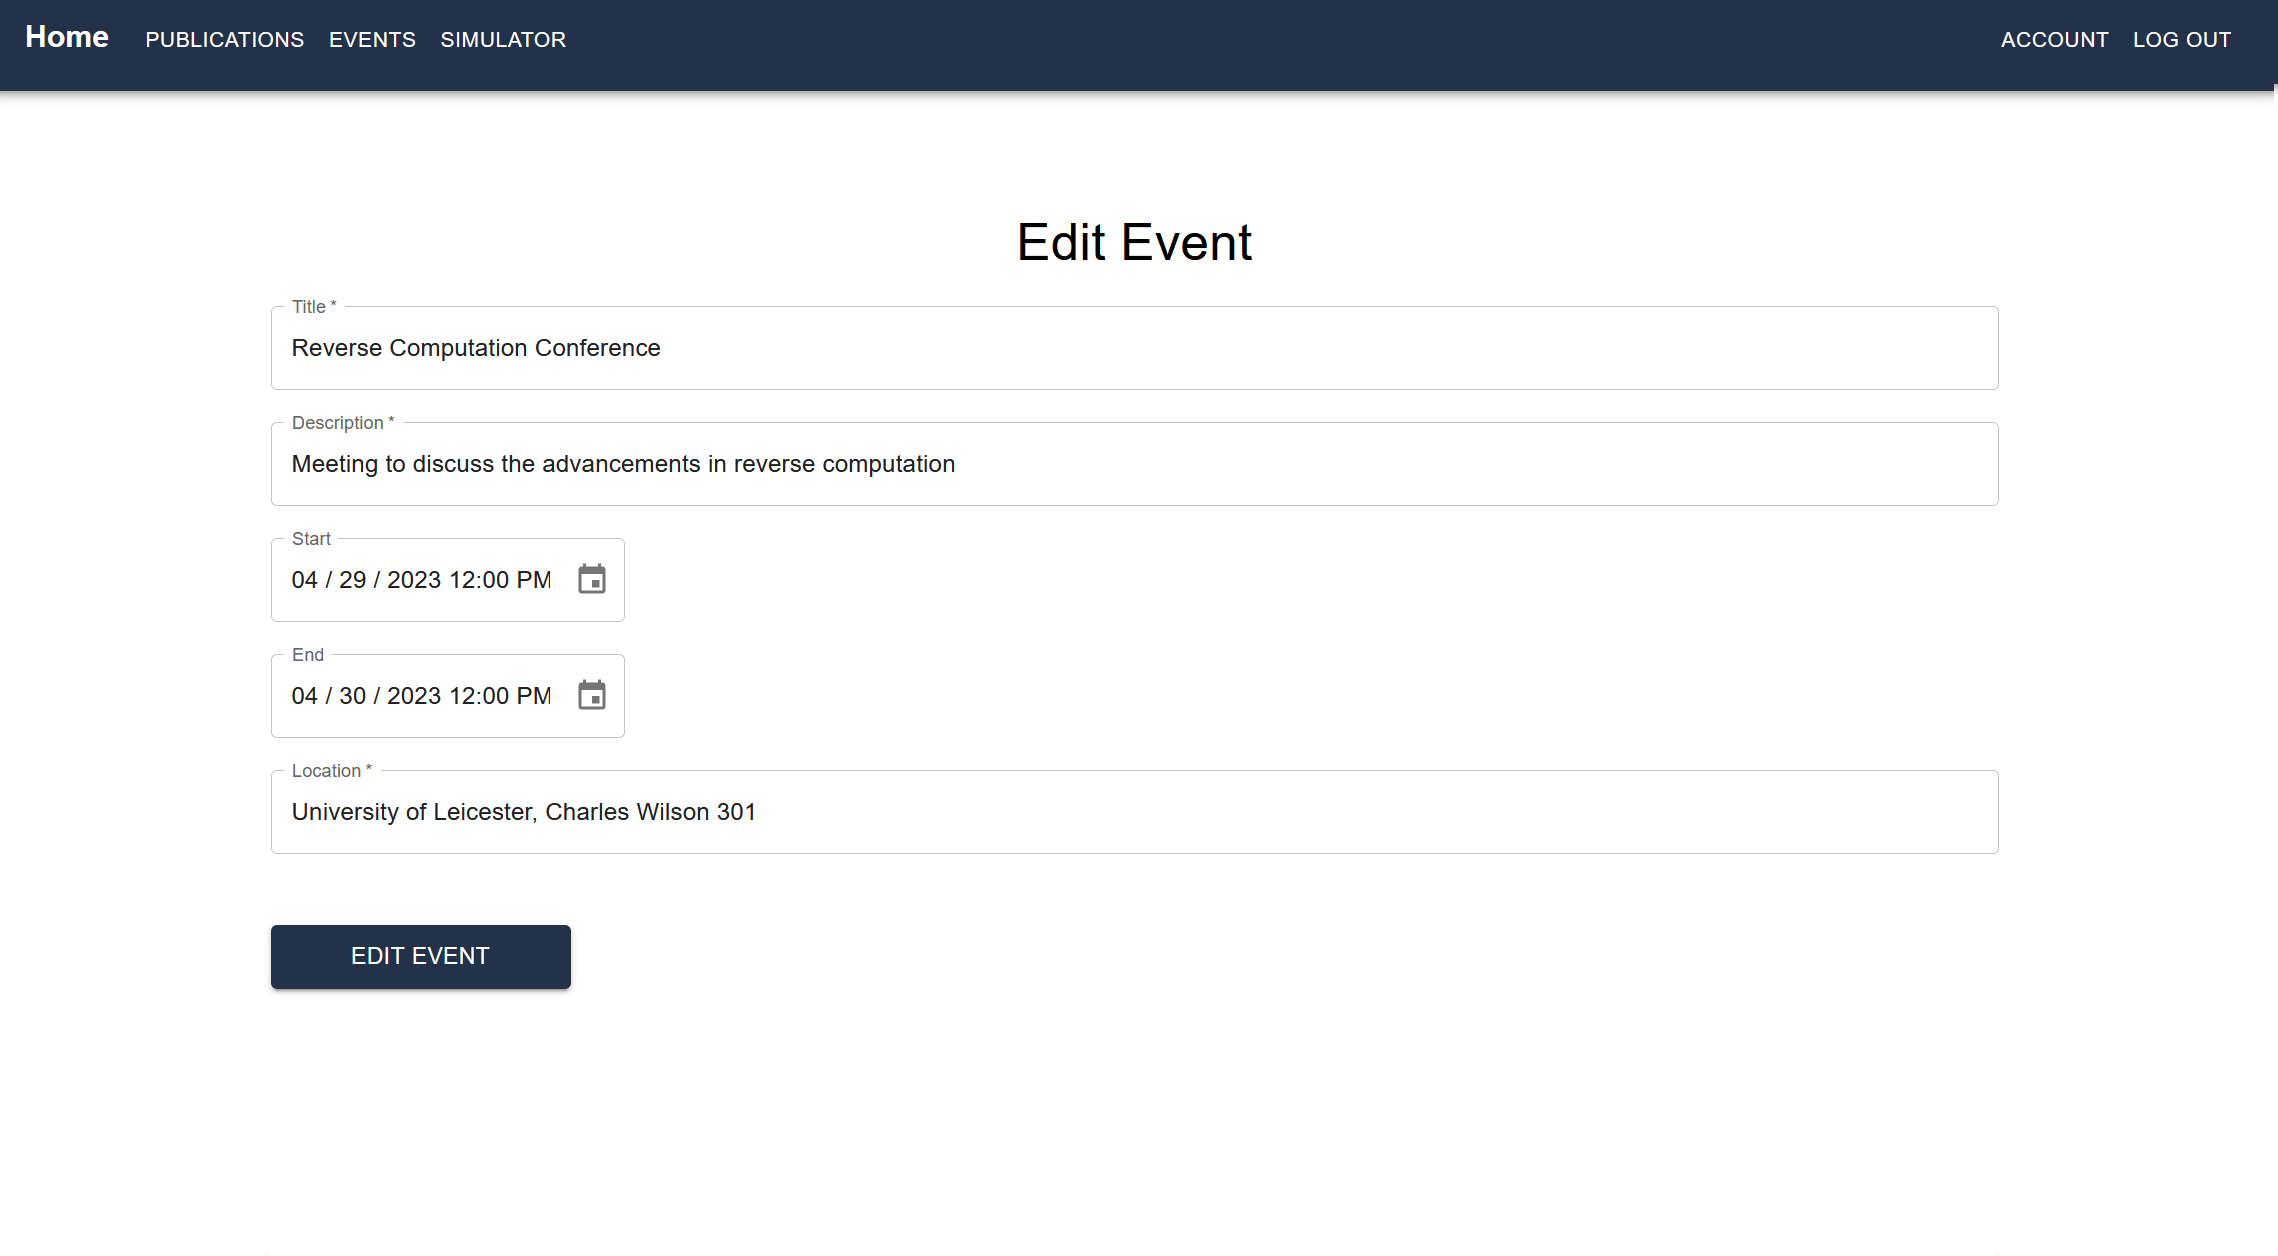
\includegraphics[width=\textwidth]{EventPageEdit2}
	\caption{Event edit page}
\end{figure}

\begin{figure}[h]
	\centering
	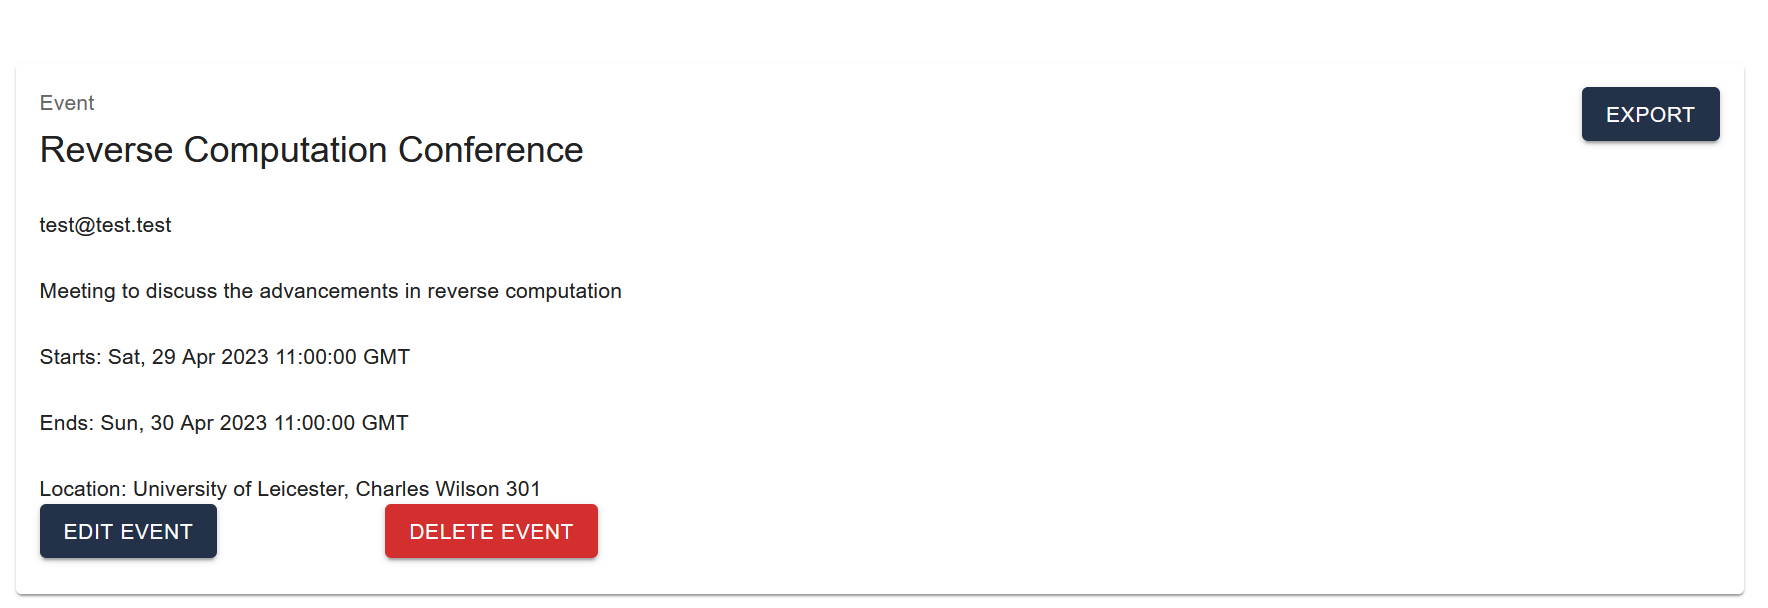
\includegraphics[width=\textwidth]{EventPageEdit3}
	\caption{Event page with updated information}
\end{figure}

\FloatBarrier
\newpage
\section{Exporting Events}

For each event, the user has the capability to export the details of the event to either Apple, Google or Outlook calendar. This can be done by the 'Export' button which can be found at the top-right of each event. Once the user clicks it they can choose the calendar of their choice and they will be redirected to the respective page with the details filled in.

\begin{figure}[h]
	\centering
	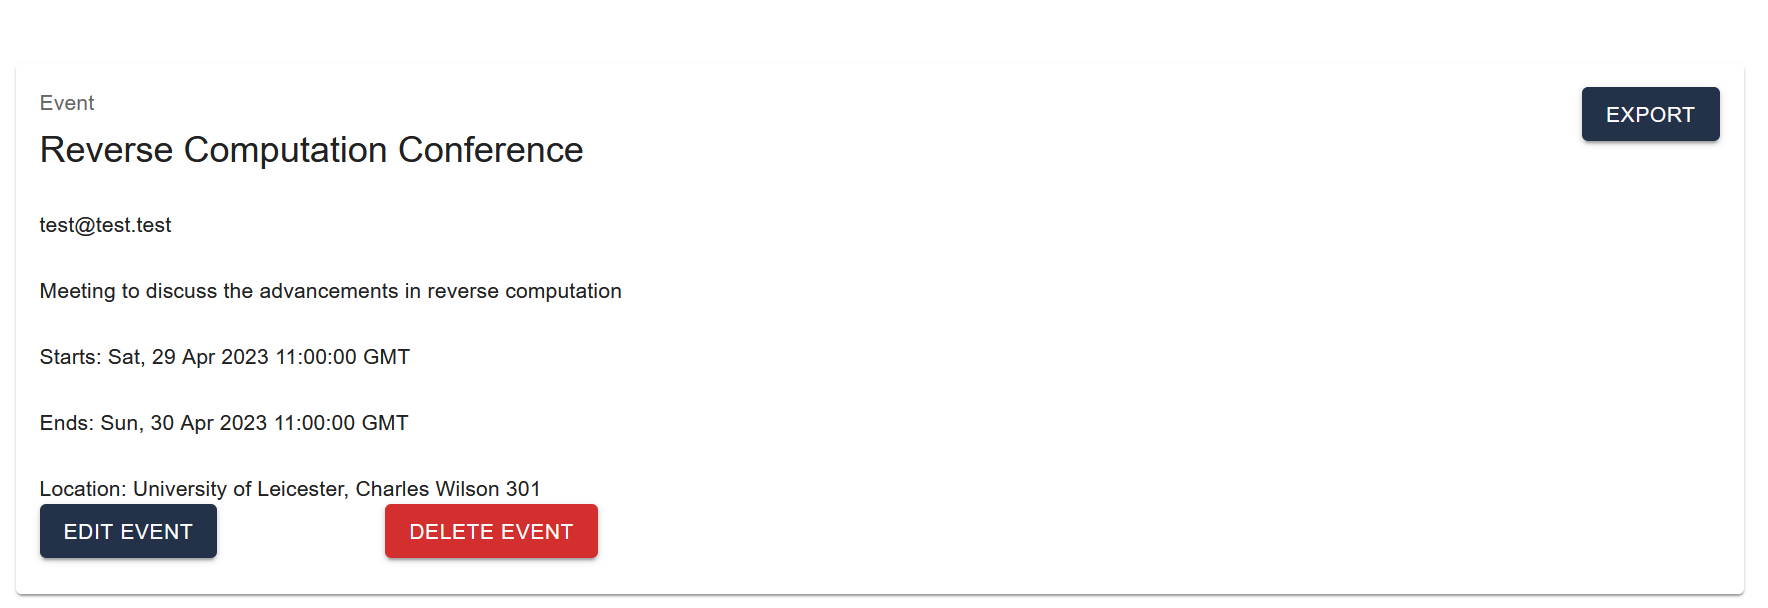
\includegraphics[width=\textwidth]{EventPageEdit3}
	\caption{Event 'Export' button on the top-right}
\end{figure}

\newpage
\chapter{Simulator}
The simulator provides all users with the ability to discover and learn about reverse computation by putting it into practice.  This is achieved by users inputting pseudocode into the simulator. They users can then instruct the simulator to take execute the code step by step in either forward of backwards direction.

\newpage
\section{Code Editor}
When the user arrives on the simulator page, they are presented with an example set of pseudo code. There is also the option to write their own code if they want.

\begin{figure}[ht]
	\centering
	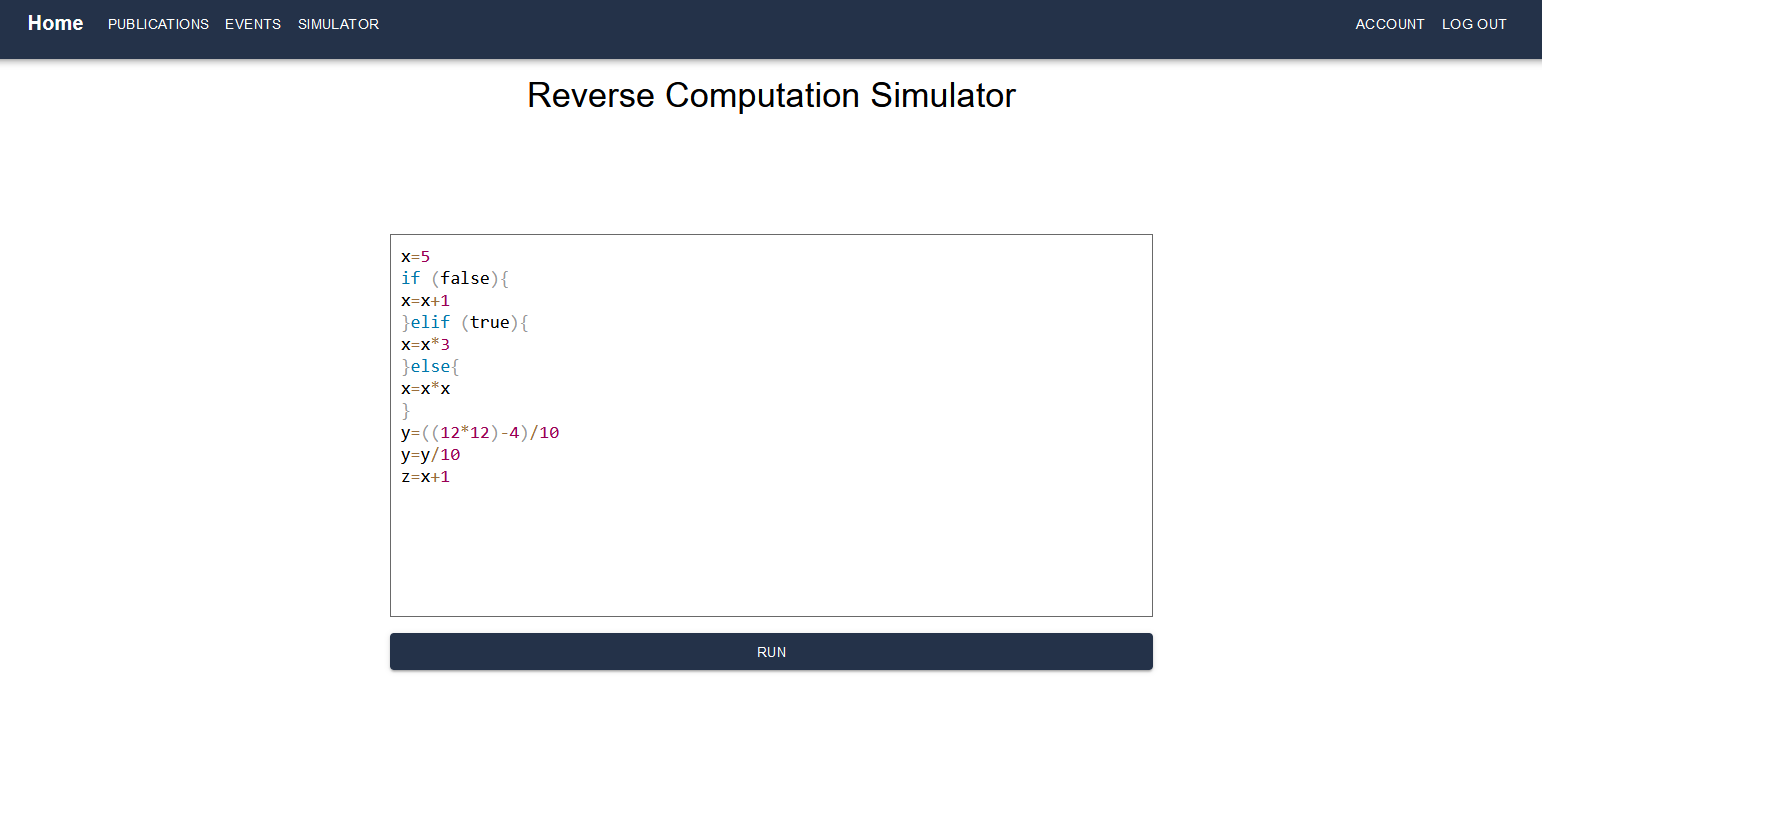
\includegraphics[width=\textwidth]{SimulatorPage}
	\caption{Example psuedocode in the editor}
\end{figure}

\newpage
\section{Code Syntax}

This section covers the complete syntax guide for the simulator.

\subsection{Variable Assignment}

Variable can be assigned in the code editor by declaring the name of a variable followed by an '=' and then the value you want to assign to the variable. Variable assignment also support arithmetic expressions.

\begin{center}
\begin{tabular}{ |c|c|c| }
	\hline
	\textbf{Operator} & \textbf{Name} & \textbf{Example} \\
	\hline
	+ & Addition & x=1+1 \\
	\hline
	- & Subtraction & x=2-1 \\
	\hline
	* & Multiplication & x=2*2 \\
	\hline
	/ & Division & x=4/2 \\
	\hline
\end{tabular}
\end{center}
	
\subsection{Comparison Operators}

The simualtor will support comparing variables against variables and constants.

\begin{center}
\begin{tabular}{ |c|c|c| }
	\hline
	\textbf{Operator} & \textbf{Name} & \textbf{Example} \\
	\hline
	== & Equal & x == 2 \\
	\hline
	!= & Not Equal & x != 1 \\
	\hline
	\textgreater & Greater then & x \textgreater 2 \\
	\hline
	\textless & Less then &  x \textless 4 \\
	\hline
	\textgreater= & Greater then or equal to & x \textgreater= 2 \\
	\hline
	\textless= & Less than or equal to & x \textless= 4 \\
	\hline
\end{tabular}
\end{center}

\subsection{Logical Operators}

You can use logical operators to perform boolean logic.

\begin{center}
\begin{tabular}{ |c|c|c| }
	\hline
	\textbf{Operator} & \textbf{Name} & \textbf{Example} \\
	\hline
	\&\& & And & x \&\& y \\
	\hline
	! & Not & !x \\
	\hline
	|| & Or & x || y \\
	\hline
\end{tabular}
\end{center}

\newpage
\subsection{If Statements}

The simulator is capable of performing 'If' statements. This allows the program to branch based off conditions that have been set in the program, written by the user. These ifs use the operators mentioned previously. 

\begin{center}
\begin{tabular}{ |p{2cm}|p{6cm}|p{3cm}| }
	\hline
	\textbf{Operator} & \textbf{Explanation} & \textbf{Example} \\
	\hline
	if & The program will run the branch if the conditions outlined are met  & if(false) \{x=x+1\} \\
	\hline
	elif & This branch will run if the previous if or elif were not run and its conditions are met & elif(true) \{x=x*3\} \\
	\hline
	else & This branch will run if the previous if or elif conditions were not met & else \{x=x*x\}\\
	\hline
\end{tabular}
\end{center}


\newpage
\section{Forward Execution}
The user can use the step buttons to execute the code line by line. The webpage will then display the current values for each of the variables that have been declared.

\begin{figure}[ht]
	\centering
	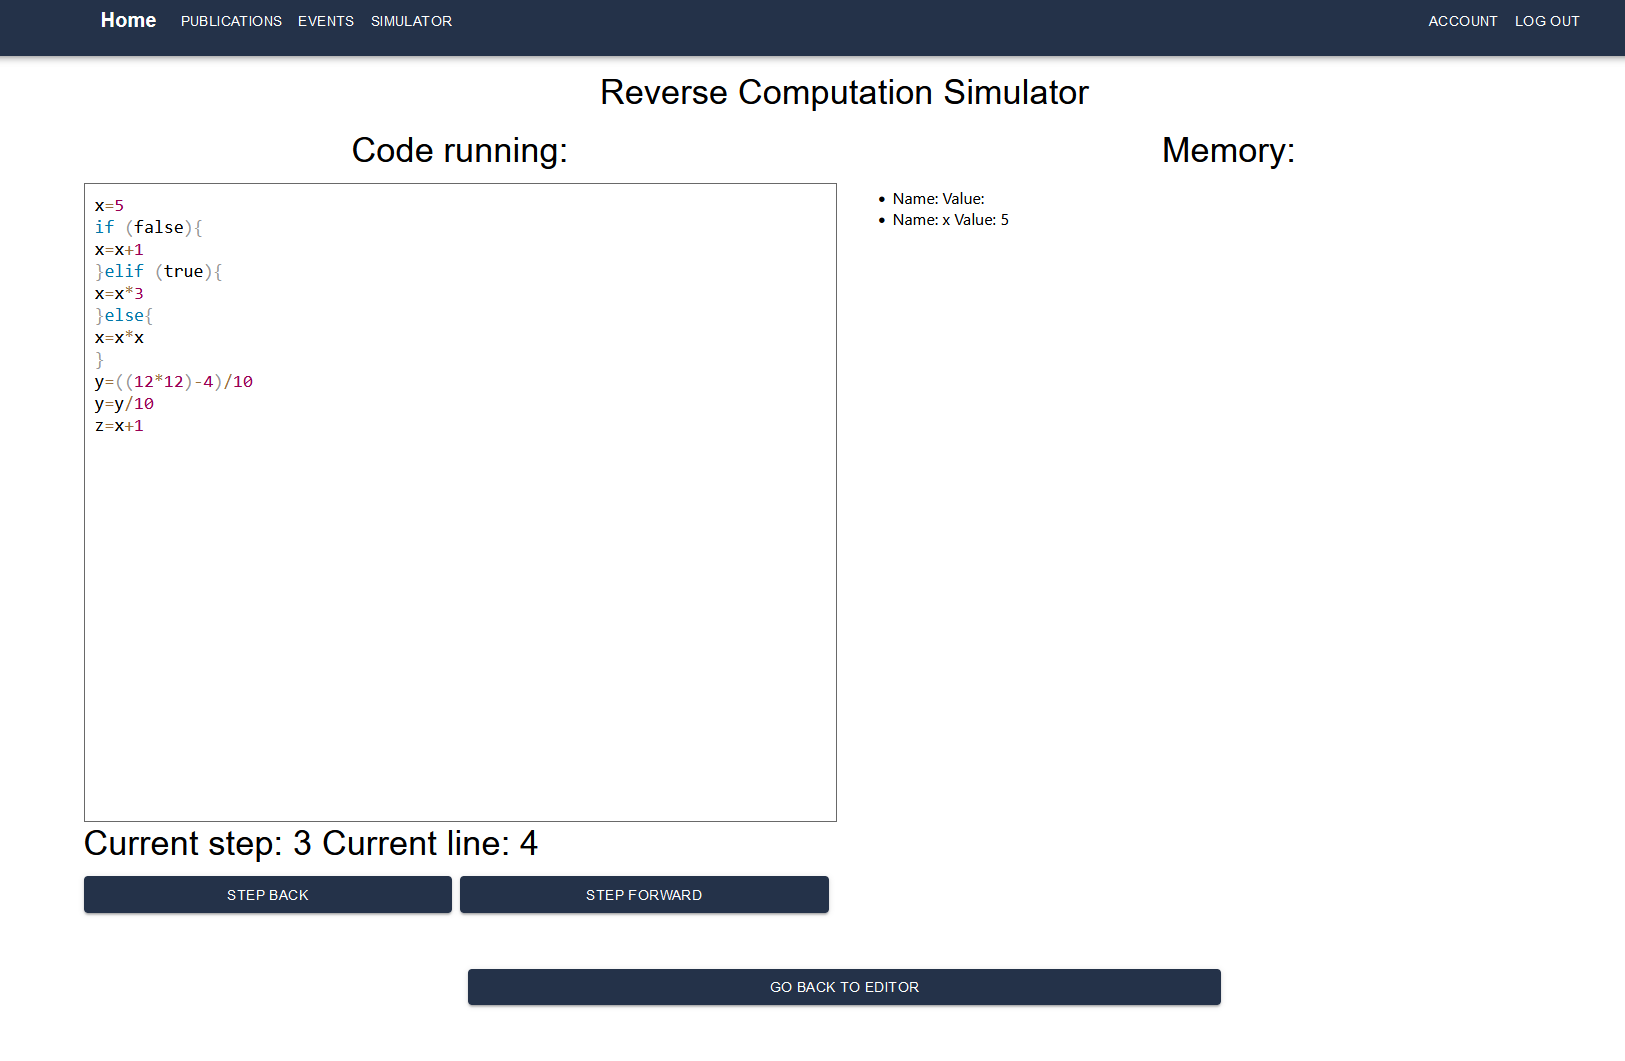
\includegraphics[width=\textwidth]{SimulatorPageForward1}
	\caption{Step 3, after three click of 'Step Forward'}
\end{figure}

\begin{figure}[ht]
	\centering
	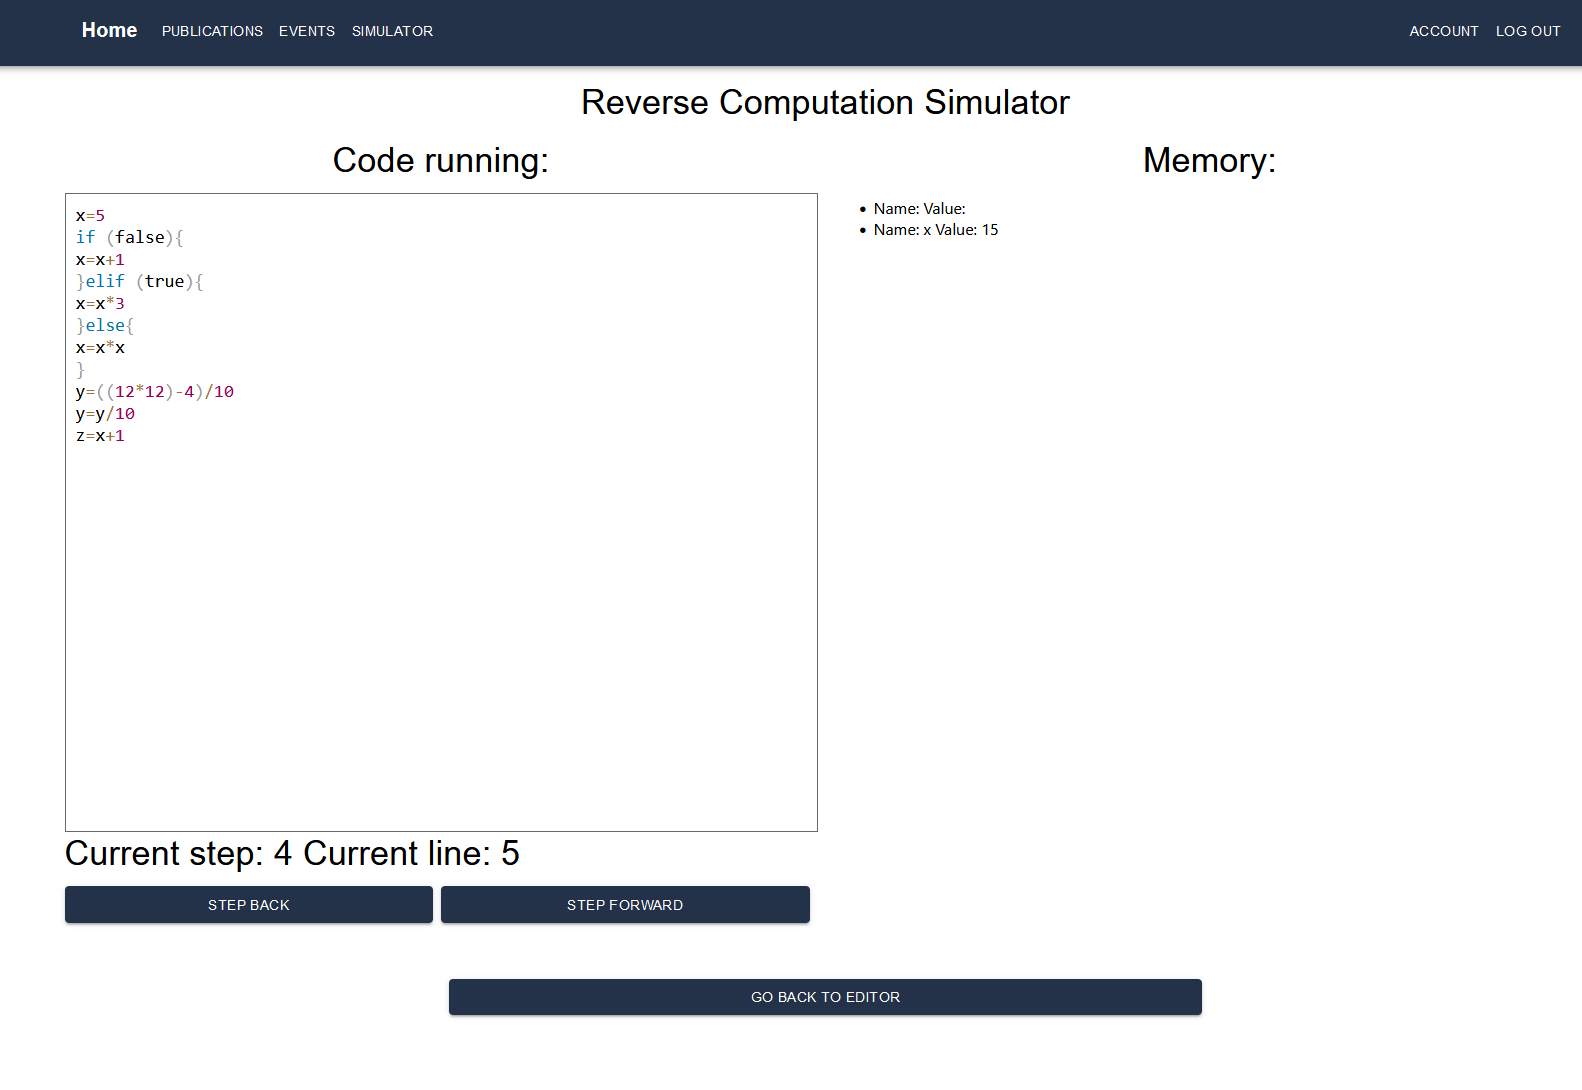
\includegraphics[width=\textwidth]{SimulatorPageForward2}
	\caption{Step 4, showing the second line of code has been executed}
\end{figure}

\newpage
\section{Reverse Executiton}
The user also has the option to execute the code in reverse. This can be achieved by clicking the 'Step Back' button

\begin{figure}[ht]
	\centering
	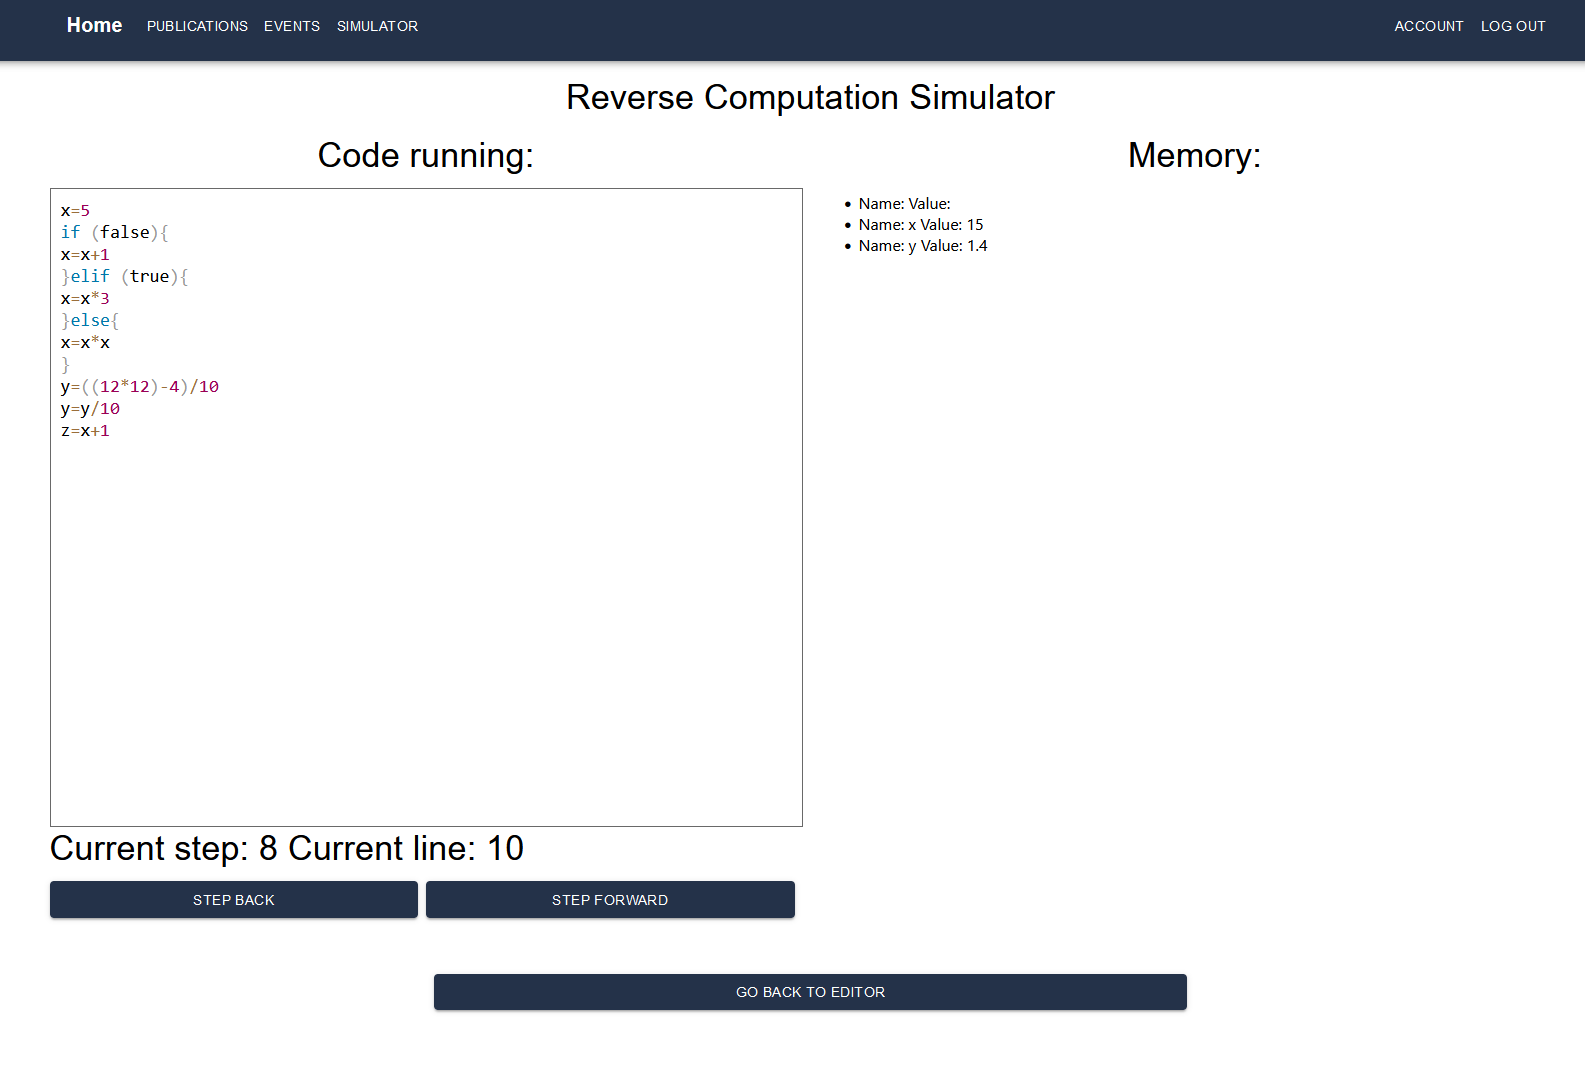
\includegraphics[width=\textwidth]{SimulatorPageBackward1}
	\caption{The program is currently at step 8}
\end{figure}


\begin{figure}[ht]
	\centering
	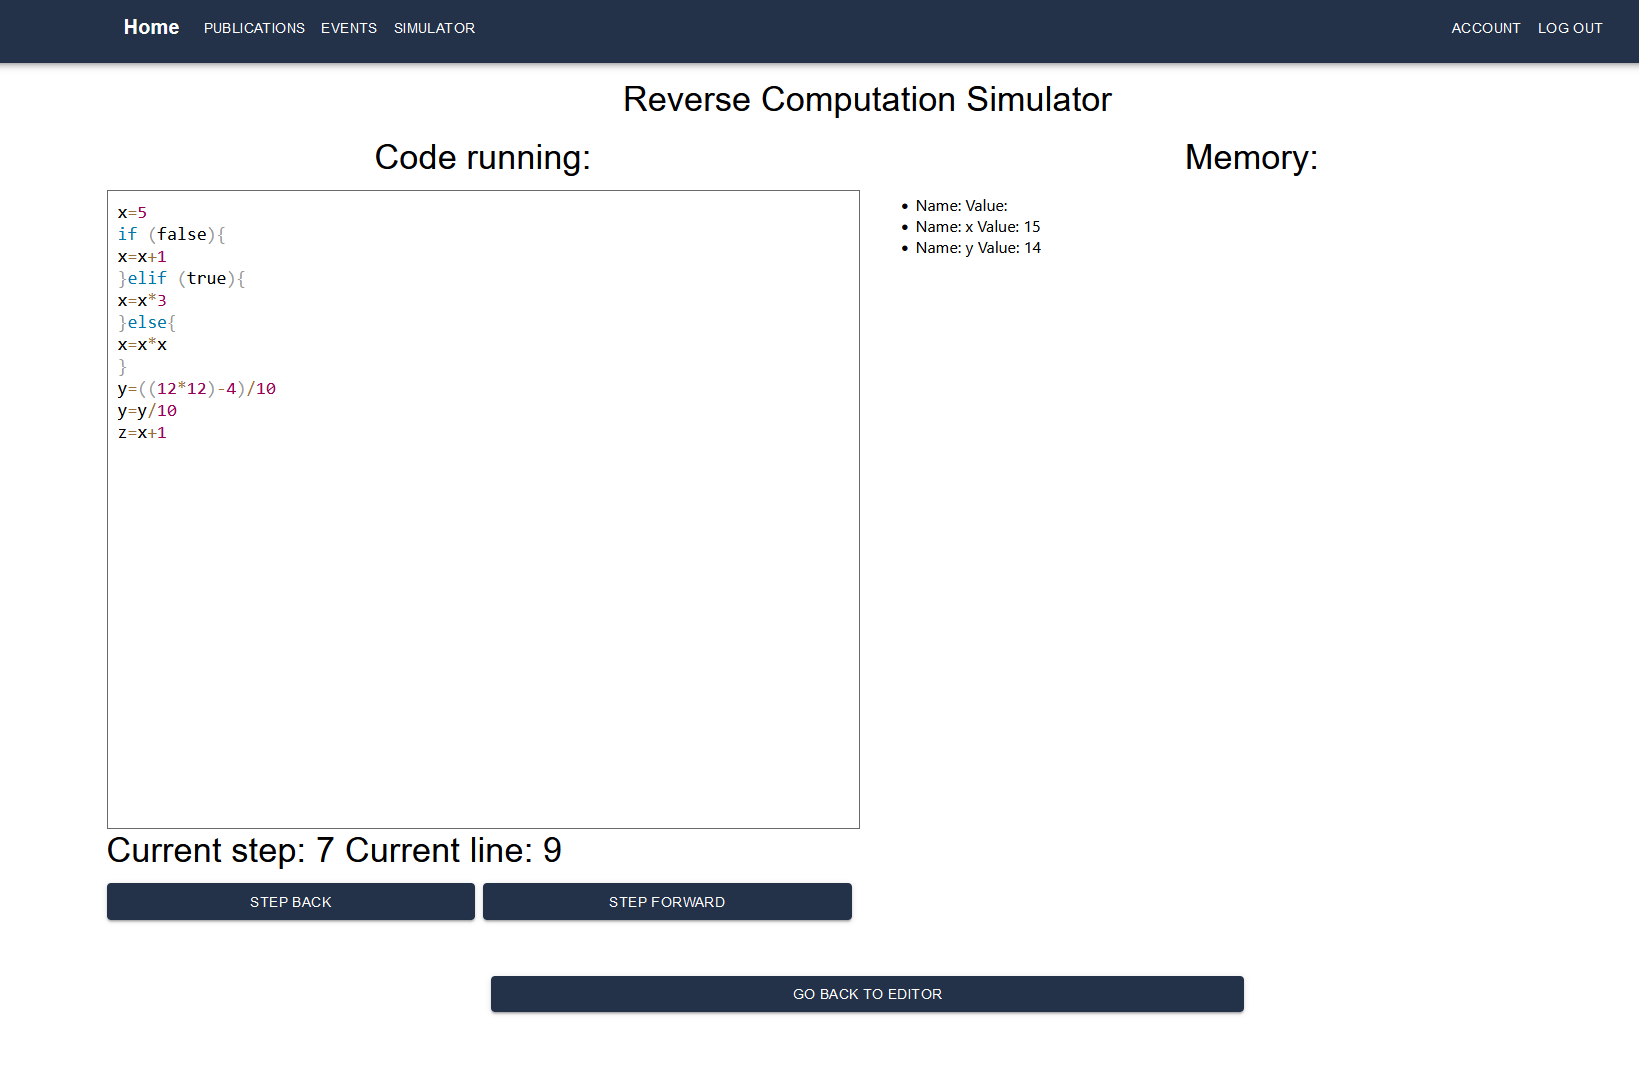
\includegraphics[width=\textwidth]{SimulatorPageBackward2}
	\caption{The program steps back to step 7}
\end{figure}

\newpage
\listoffigures
\end{document}